% Inserts the customizations
\documentclass [11pt,twoside,english]{article}
\usepackage[utf8]{inputenc}
\usepackage[T1]{fontenc}

% Page margins, header and footer positions
\usepackage{geometry}
\geometry{
	a4paper,
	total={210mm,297mm},
	left=25mm,
	right=25mm,
	top=30mm,
	bottom=25mm,
	headsep=7mm
}

\interfootnotelinepenalty=10000

%To display filling dots in the TOC for all entries
\usepackage[titles]{tocloft}
\renewcommand{\cftsecleader}{\cftdotfill{\cftdotsep}}

%Define new header and footer style
\usepackage{fancyhdr}

\pagestyle{fancy}
\fancyhf{}
\lhead{\color{Gray}{\small{CLup project}}}
\lfoot{\textcolor{Gray}{\small{Copyright © 2020 – All rights reserved}}}
\rfoot{\textcolor{Gray}{\thepage}}
\renewcommand{\headrulewidth}{0pt}

% PACKAGES
\usepackage{wasysym}
\usepackage{pifont}

\newcommand{\supported}{\ding{52}\xspace}
\newcommand{\unsupported}{\ding{55}\xspace}
\newcommand{\partsupported}{\textcolor{black!40}{\ding{52}}\xspace}
\newcommand{\lowsupported}{\textcolor{black!20}{\ding{52}}\xspace}
\newcommand{\unknowsupported}{\textbf{?}\xspace}

%Font: Times
\usepackage{times}
%Change monospaced font
\renewcommand{\ttdefault}{lmtt}

% Tables
\usepackage{tabu}
\usepackage{tabularx}
\usepackage{ltablex}
\usepackage{longtable}
\usepackage{float} % To allow the use of H modifier in long tables
\usepackage{multirow}

% Landscape mode
\usepackage{pdflscape}
\usepackage{rotating}
\usepackage{caption}

% Graphics and images
\usepackage{graphicx}
\usepackage[dvipsnames, table]{xcolor}
\graphicspath{{./images}}
\usepackage{subcaption}

%References
%\usepackage{xpatch}
%\usepackage[backend=biber, style=numeric, citestyle=numeric, sorting=none]{biblatex}
%\addbibresource{main.bib}

%Other
\usepackage{ifthen}
\usepackage{xspace}
\usepackage{enumitem}
\usepackage{amssymb}
\usepackage[pdftex, colorlinks]{hyperref}

% Use normal apostrophe when writing code
\usepackage{upquote}

% Alloy related packages
\usepackage{listings}
\usepackage{accsupp}

% Tables-related commands
\definecolor{tablerow}{RGB}{240, 240, 240}
\definecolor{tableborder}{RGB}{150,150,150}
\setlength{\tabcolsep}{12pt}
\arrayrulecolor{tableborder}

% Hyperlinks setup
\hypersetup {
	linkcolor=Black,
	urlcolor=MidnightBlue,
	citecolor=Black
}

% Section and subsection coloring
\usepackage{titlesec}

\titleformat{\section}
{\color{Blue}\normalfont\LARGE\bfseries}
{\color{Blue}\thesection}{1em}{}

\titleformat{\subsection}
{\color{Blue}\normalfont\Large\bfseries}
{\color{Blue}\thesubsection}{1em}{}

\titleformat{\subsubsection}
{\color{Blue}\normalfont\large\bfseries}
{\color{Blue}\thesubsubsection}{1em}{}

\date{}



\begin{document}
	
	% Front page
	\begin{titlepage}
		
		% PoliMI logo
		\centering
		\includegraphics[scale=0.3]{Logo_Politecnico_Milano}
		
		% Description
		\Large 
		A.Y. 2020/2021
		
		Computer Science and Engineering
		
		\LARGE
		Software Engineering 2 Project
		\\ [3cm]
		
		% Title, maybe use an image
		\textbf{\color{Blue} \Huge CLup - Customers Line-up}
		
		% Subtitle
		Requirement Analysis and Specification
		Document
		\\ [1cm]
	
		% Authors
		\Large
		\begin{tabu}{ccccc}
			& - & & - & \\
			& - & & - & \\
			& - & & - & 
		\end{tabu}
	
	% Should place somewhere the logo
	\end{titlepage}
	
	% Table for deliverable-specific info
	\begin{table}[h!]
		\begin{tabu} to \textwidth { X[0.3,r,p] X[0.7,l,p] }
			\hline
			\textbf{Deliverable:} 	& RASD\\
			\textbf{Title:} 		& CLup - Requirement Analysis and Verification Document \\
			\textbf{Authors:}		& \\
			\textbf{Version:} 		& 1.0 \\ 
			\textbf{Date:} 			& 2020-12-22 \\
			\textbf{Download page:} & \href{https://github.com/rb-sl/SoftEng2Project2020}{https://github.com/rb-sl/SoftEng2Project2020} \\
			\textbf{Copyright:} 	& © 2020 – All rights reserved \\
			\hline
		\end{tabu}
	\end{table}
	
	\setcounter{page}{2}
	
	% Pages for table of contents and lists
	\newpage	
	\addcontentsline{toc}{section}{Table of Contents}
	\tableofcontents
	
	\newpage
	\addcontentsline{toc}{section}{List of Figures}
	\listoffigures
	
	% Introduction section
	\clearpage
	% Introduction page, to be included in dd.tex

\section{Introduction}
\label{sect:intro}

\subsection{Purpose}
This document represents the DD (Design Document) of the CLup application; it describes CLup's architecture and integrates with the RASD. Furthermore, it describes its components, how they interact, and what is the plan for implementation, integration and testing.

\subsection{Scope}
\subsubsection{Problem description}
CLup is a software-to-be that will help stores and customers preventing dangerous crowds during shopping due to the current Covid-19 Pandemic. This system should offer the possibility to line up from home for stores while still allowing to physically line up for stores. Moreover, it should offer the possibility to book a visit for a chosen store and get notifications about stores occupancy during the week.
The system should also allow store managers to add their stores to the system and monitor entrances.

The application has to be easy-to-use, scalable and reliable.

\input{introduction/definitions}

\subsection{Revision history}
\begin{center}
	\begin{tabular}{c | c | c}	
		Version & Date & Comment \\ \hline
		1.0 & 2021-01-03 & First release
	\end{tabular}
\end{center}

\subsection{Reference documents}
R\&DD Assignment AY 2020-2021, \textit{Software Engineering 2's BeeP page}

\subsection{Document structure}
This document is composed of the following parts:
\begin{itemize}[itemsep=-1mm, topsep=-1mm]
	\item \textbf{Section \ref{sect:intro}} is an introduction to the document and offers an overview of the document
	\item \textbf{Section \ref{sect:arch}} describes the application design, showing its components and explaining the design decisions
	\item \textbf{Section \ref{sect:ui}} shows the user interface diagrams of the application
	\item \textbf{Section \ref{sect:trace}} maps the requirements identified in the RASD to the components described in section \ref{sect:arch}
	\item \textbf{Section \ref{sect:iit}} suggests an implementation and test strategy 
	\item \textbf{Section \ref{sect:effort}} reports the effort spent and the tools used to realize this document	
\end{itemize}
	
	% Description section
	\clearpage
	% Description section, to be included in RASD.tex

\section{Overall Description}
\label{sect:overview}

\subsection{Product perspective}
The application's users will be able to interact through either mobile apps or web-based applications (predominantly with an interface optimized for mobile devices).

When used by customers, the system will need to use a web mapping service such as Google Maps to provide a position (if needed) and calculate travel times.

On the other hand, when used in stores, it will need to be connected to QR code readers (either mobile devices or dedicated scanners) ticket printers, and screens.

% Scenarios file, to be included in overview.tex

\subsubsection{Scenarios}
The following scenarios are provided to describe possible situations during the usage of CLup.

\paragraph{Scenario 1}
Nathan, during the pandemic, needs a way to safely go grocery shopping, avoiding long queues out of supermarkets. His friend John suggests him to download the CLup app to line up from home; Nathan is intrigued and immediately downloads it, signs up and enqueues for his favorite shop.

\paragraph{Scenario 2}
After being enqueued for about thirty minutes, Nathan receives a notification telling him his turn is close and he needs to leave home. After reaching the supermarket he waits for some minutes until his number gets displayed by the shop; he then passes the QR code shown by the application at a scanner and enters the shop. Once he has done, he scans again the code at the exit and goes home. 

\paragraph{Scenario 3}
Ms. Margareth is not accustomed to technology, so she does not use a smartphone; as she needs to go grocery shopping, she goes directly to the store and gets a physical ticket, so she can wait outside with few people, as most use CLup. Once she sees her number is reached, she scans the ticket and enters.

\paragraph{Scenario 4}
Nathan knows Julie, the owner of a bakery close to his house, so he tells her about CLup. She is curious and downloads the app, registering her shop. She then logs in as Store Manager into the tablet she uses for work, so that her employees can use it to scan codes and monitor the entrance of customers.

\paragraph{Scenario 5}
Anthony works for a supermarket that adopted CLup. As a store manager, he has the duty of keeping updated the store’s inventory and make customers respect their turns. Luckily, the store decided to install some QR code readers connected to CLup at entrances, so he doesn’t have to scan every customer’s code himself. 

\paragraph{Scenario 6}
As Joe had some free time, he decided to get a physical ticket for the supermarket, hoping few people were already lined up. After 10 minutes of being enqueued he receives an important call and needs to leave; he decides to scan his ticket to dequeue and let the people behind him enter some time before.

\paragraph{Scenario 7}
Andrew is at home, waiting for his turn after he requested a ticket. Suddenly he receives a notification from CLup, letting him know that someone in front of him dequeued and giving him the possibility to enter earlier than expected. He gladly accepts and gets ready to go.

\paragraph{Scenario 8}
Anastasia knows she needs to go shopping for groceries the next day but has a very tight schedule. Luckily, she can use CLup to book a visit for the exact time she chooses, so she requests a reservation. The next day she can enter without having to line up, thus saving much of her time.

\paragraph{Scenario 9}
Confident about his free time, Nick booked three visits for the next week. The day before the second one he remembered he was actually busy, so he logged in the application and canceled the reservation.

\subsection{Product functions}
The major objective of the application is to decrease queues outside stores; this is achieved by allowing customers to line up from home and book visits for specific dates and times. These functions are integrated with alerts telling the user when to leave home, along with possibility to subscribe to notifications about store occupancy throughout the week to better plan store visits.

For customers not using the application, options to take physical tickets and wait outside store are offered.

\subsection{User characteristics}
Due to the nature of the application, users can span a wide variety of people with different needs of accessibility and functions.

\subsubsection{Actors}
Actors represent the groups of people that interact with the application. The relations among the active actors are shown in Figure \ref{actors}.
\begin{itemize}[itemsep=-1mm, topsep=-1mm]
	\item \textbf{Prospective e-Customer}: A person who would like to use the application as customer
	\item \textbf{Prospective Store Manager}: A person who would like to register their store
	\item \textbf{Physical Customer}: A customer not registered to the application
	\item \textbf{e-Customer}: A customer using the application
	\item \textbf{Store Manager}: A user managing a store
\end{itemize}

\begin{center}
	\begin{figure}[h]
		\centering	
		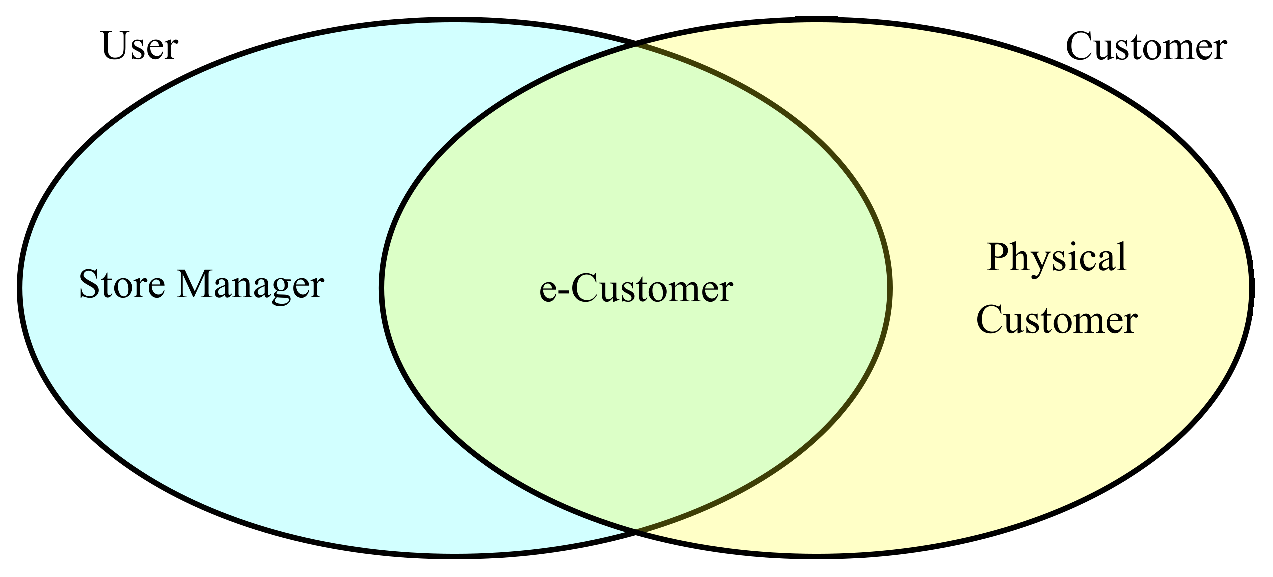
\includegraphics[width=.7\textwidth] {actors}
		\caption{Active actor relations}
		\label{actors} 
	\end{figure}
\end{center}

\subsection{Assumptions, dependencies and constraints}

\subsubsection{Text assumptions}
Due to the ambiguity created by the natural language, we made the following assumptions about the specification.

\begin{itemize}[itemsep=-1mm, topsep=-1mm]
	\item For each store exists only one store manager; this way, if more people need to use the functions they will need an already logged in terminal
	\item Some places in stores will need to be reserved to tickets, both in their physical and virtual form, to avoid creating situations where reservations monopolize the entrances
	\item QR codes will need to be scanned both at entrance and exit, in order to better know the store's occupation and how much time customers spend inside
\end{itemize}

% File for domain assumptions, to be included in overview.tex

\subsubsection{Domain assumptions}

\begin{itemize}[itemsep=-1mm, topsep=-1mm]
	\item [\textbf{[D0]}] Prospective users will complete the registration process
	\item [\textbf{[D1]}] Only people enqueued access the stores (both app and physical)
	\item [\textbf{[D2]}] Information provided by e-customers corresponds to their will
	\item [\textbf{[D3]}] Information provided by users upon registration is correct
	\item [\textbf{[D4]}] Customers enter only if allowed by the application
	\item [\textbf{[D5]}] Customers respect the choices made during a ticket creation or while booking a visit
	\item [\textbf{[D6]}] Calculated travel time is correct
	\item [\textbf{[D7]}] Information about stores inserted by SMs is correct
	\item [\textbf{[D8]}] Customers entering a store exit after some time
	\item [\textbf{[D9]}] If a client exits at a given time, he must have entered in the same opening period
	\item [\textbf{[D10]}] Ticket printers and QR readers work properly
	\item [\textbf{[D11]}] The internet connection is always working
	\item [\textbf{[D12]}] Users accept to receive notifications from the application
	\item [\textbf{[D13]}] Stores show the current customer number
	\item [\textbf{[D14]}] The external web mapping system is always available and there is signal
\end{itemize}

\newpage
\subsection{Domain Diagrams}
The high-level class diagram of the application can be seen in Figure \ref{class}, while Figure \ref{ticket_state} contains the state diagram for tickets; the beginning of the $CanEnter$ state corresponds to the start of the delay window. Figure \ref{open_store} shows the acceptance states of a store during its opening hours.

\begin{center}
	\begin{figure}[h]
		\centering	
		\includegraphics[width=0.9\textwidth] {state_diagrams/ticket}
		\caption{Ticket state diagram}
		\label{ticket_state} 
	\end{figure}
\end{center}

\begin{center}
	\begin{figure}[h]
		\centering	
		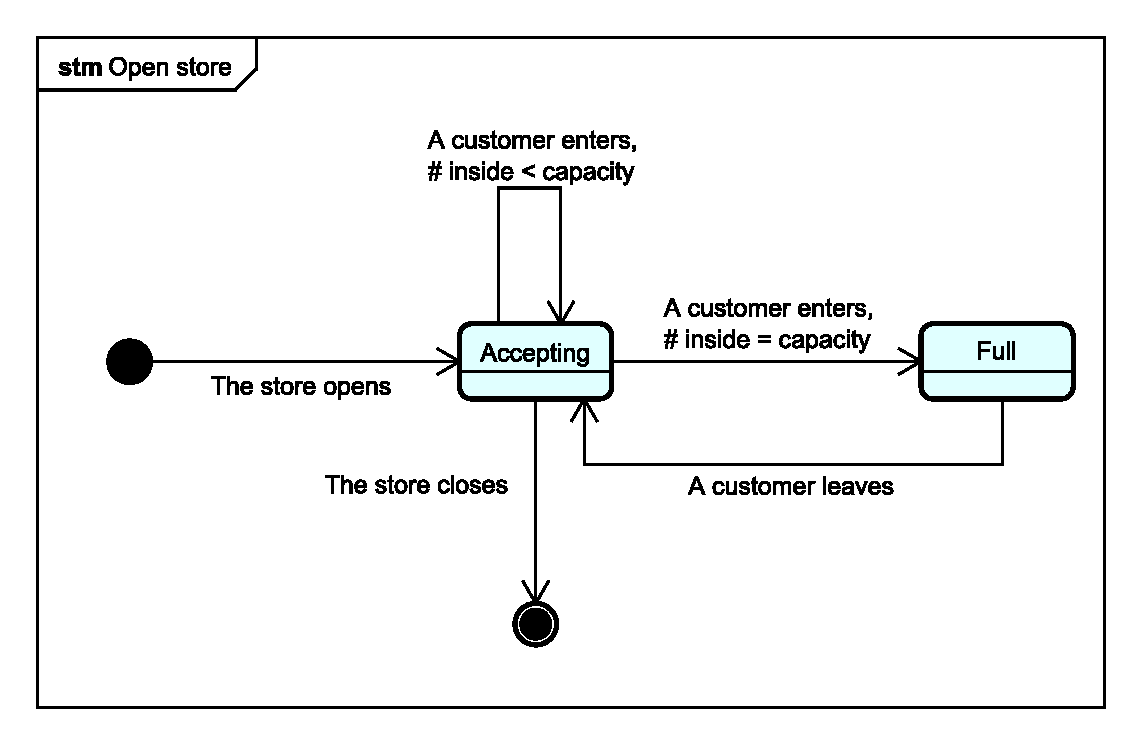
\includegraphics[width=0.9\textwidth] {state_diagrams/open_store}
		\caption{Open store diagram}
		\label{open_store} 
	\end{figure}
\end{center}

\begin{landscape}
	\begin{figure}[hp]
		\centering	
		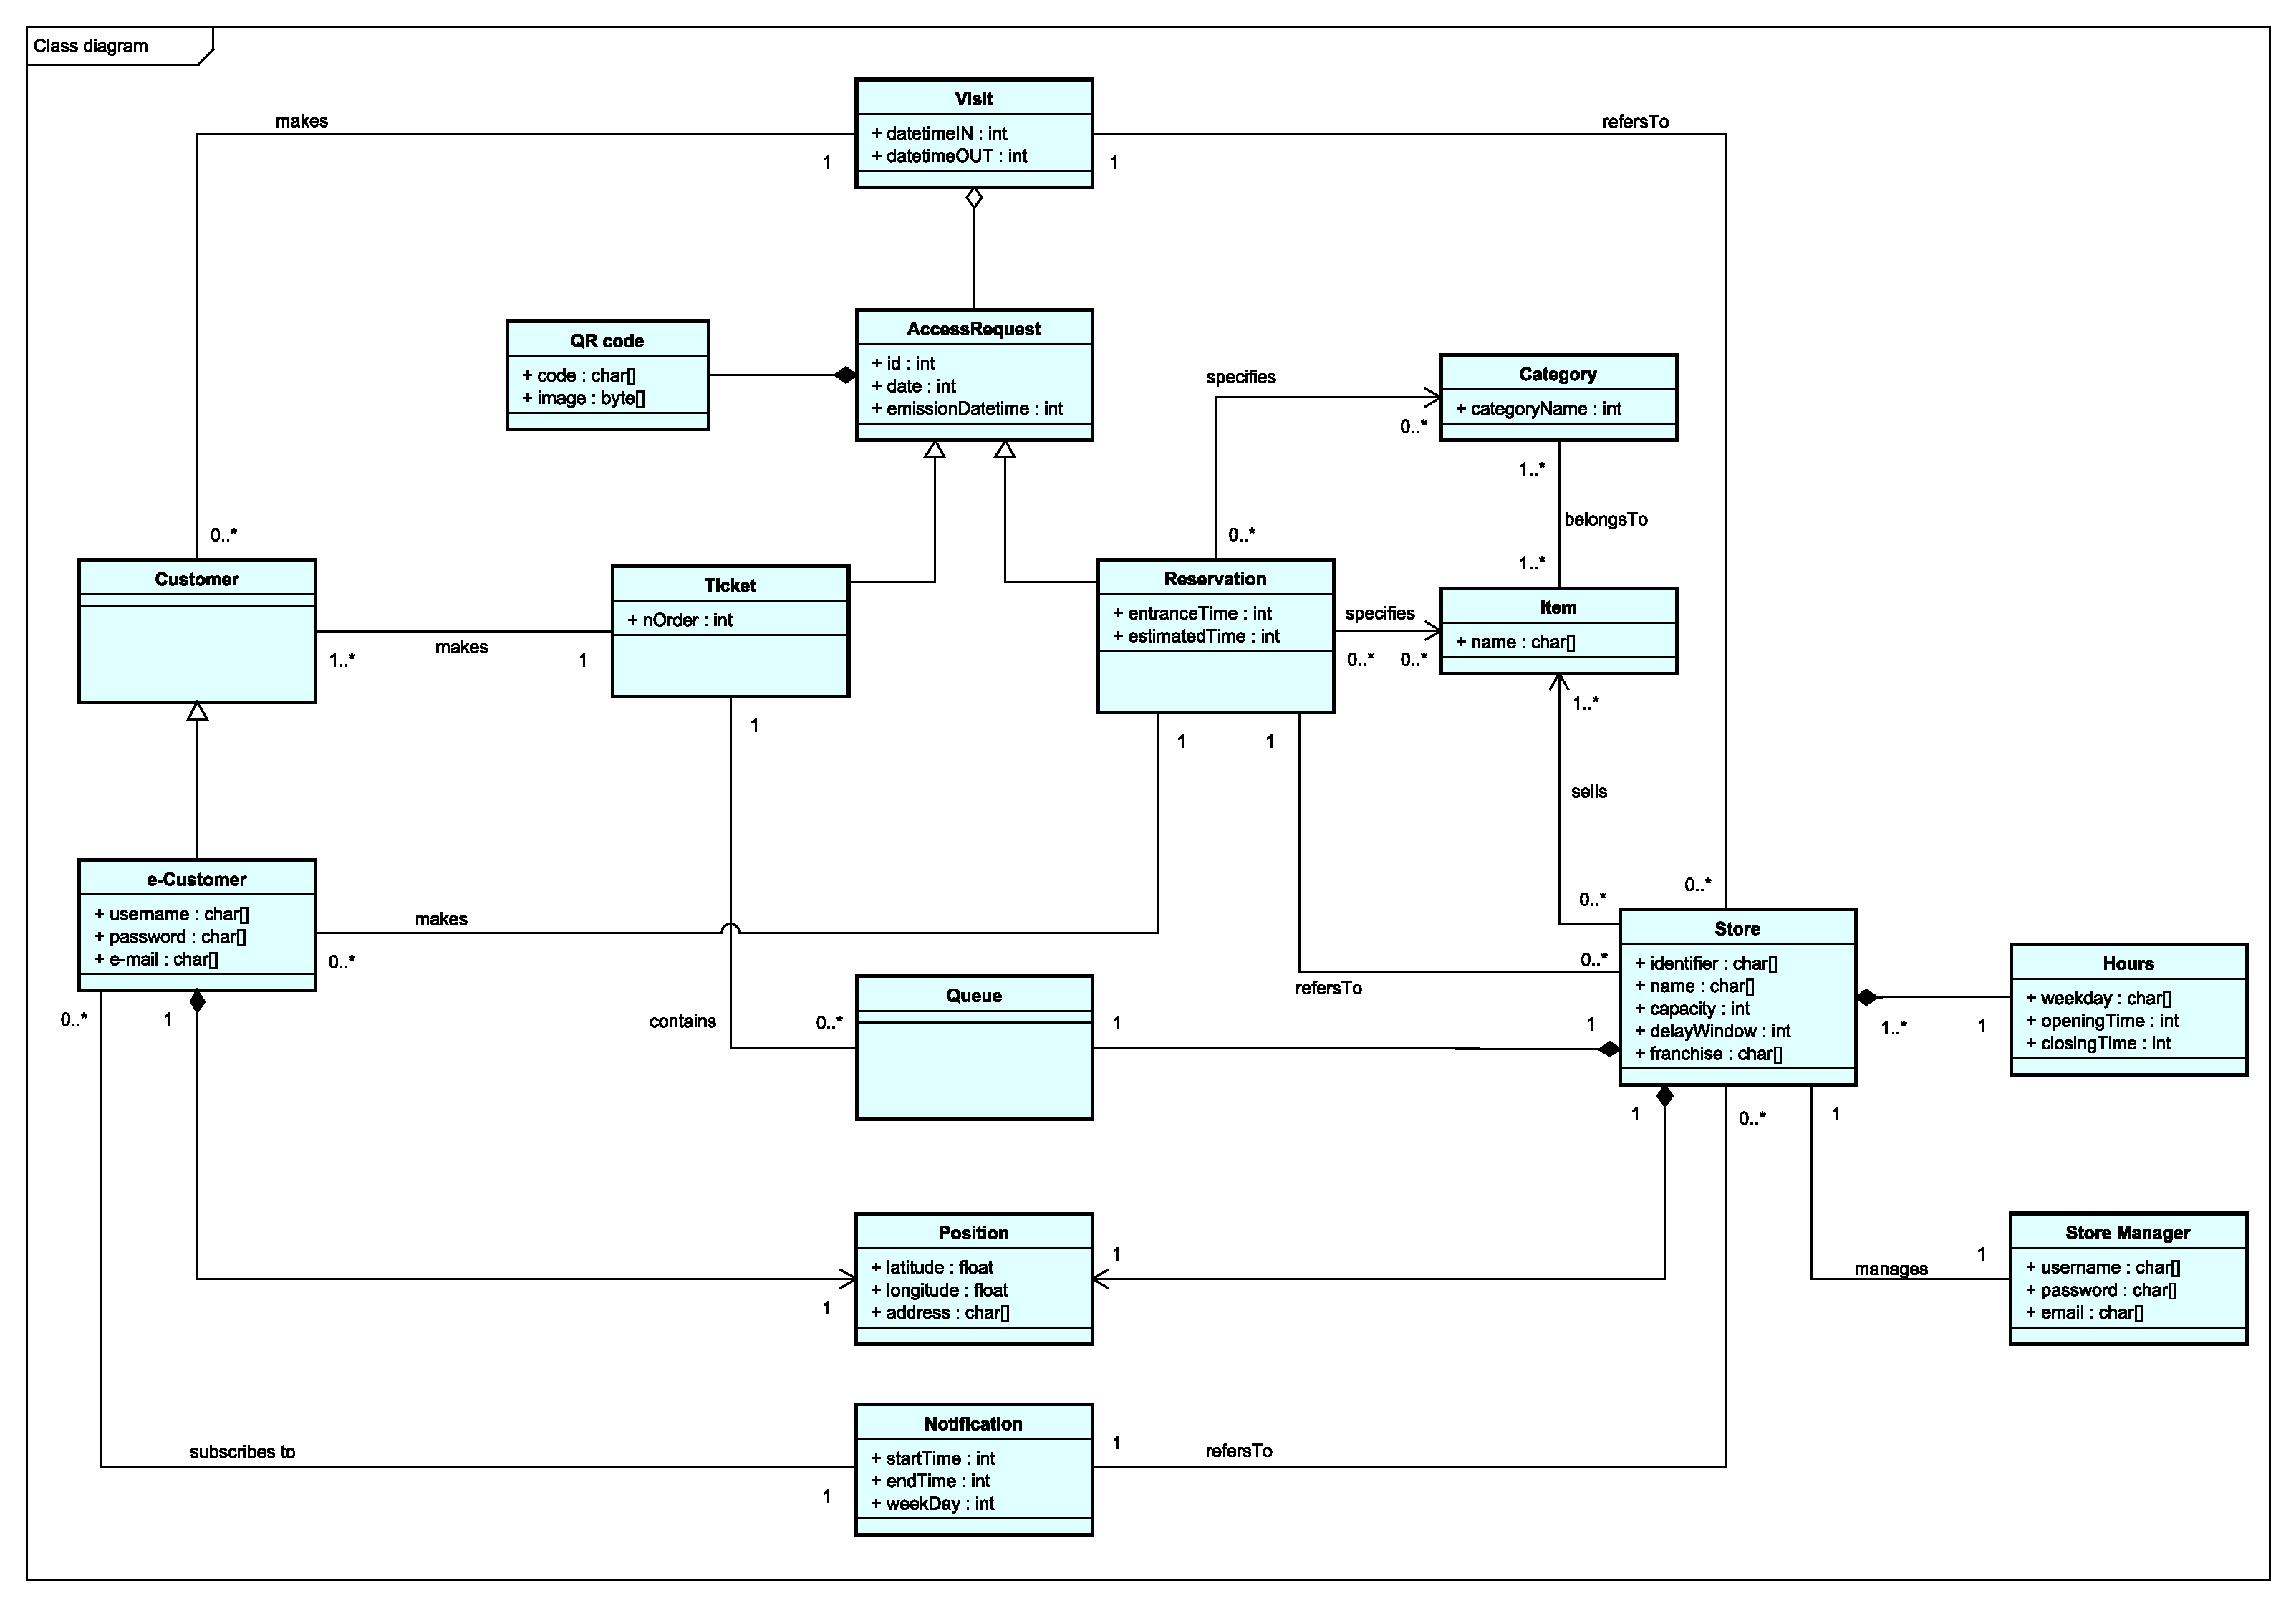
\includegraphics[height=\textheight] {class}
		\caption{Class Diagram}
		\label{class} 
	\end{figure}
\end{landscape}

	
	% Requirements section
	\clearpage
	% Requirements section, to be included in RASD.tex

\section{Specific Requirements}
\label{sect:requirements}

\subsection{External interface requirements}

% User interface design section, to be included in dd.tex

\section{User interface design}
\label{sect:ui}
This section illustrates the UX diagrams, i.e. the transitions between the user interface's pages. The application's mock-ups can be found in the RASD.

\subsection{e-Customer UX diagram}
The e-Customer application is composed of four sections reachable through tabs:
\begin{itemize}[itemsep=-1mm, topsep=-1mm]
	\item Home page: displays some instructions to better explain the application's interfaces and functions, and how to navigate through them. Moreover, it shows the active access requests (if present)
	\item Ticket creation: allows the user to line up by filling the creation form and then choosing a store among the suggested ones
	\item Book a visit: allows the e-Customer to create a new reservation by passing through the three booking form steps and then by choosing the store they like from the list of the ones meeting the specified parameters
	\item Settings: allows e-Customers to manage notifications, subscriptions and their profile
\end{itemize}\vspace{.5\baselineskip}

These sections can be reached after the login or signup process Figure \ref{uxec} shows the transitions.

\begin{figure}[h]	
	\centering
	\includegraphics[width=\linewidth] {ux_diagrams/eCustomer_UX}
	\caption{UX diagram of the e-Customer application}
	\label{uxec} 
\end{figure}

\newpage
\subsection{Store Manager UX diagram}
The Store Manager application is composed of four sections as well:
\begin{itemize}[itemsep=-1mm, topsep=-1mm]
	\item Home page: displays instructions about the application's functionalities and gives the possibility to access other functions such as viewing store statistics or modifying the store's parameters
	\item Ticket creation: allows the Store Manager to see the enqueued tickets and to create and print physical ones
	\item Reservations: allows the Store Manager to visualize active reservations by date
	\item Settings: allows Store Manager to change information related to their profile
\end{itemize}\vspace{.5\baselineskip}
These sections can be reached after a login or signup process ended up successfully; furthermore, every screen can activate the QR code scanning function. Figure \ref{uxsm} shows the transitions 
among the interfaces.

\begin{figure}[h]	
	\centering
	\includegraphics[width=\linewidth] {ux_diagrams/StoreUX}
	\caption{UX diagram of the Store Manager application}
	\label{uxsm} 
\end{figure}


\subsubsection{Hardware interfaces}
On the e-Customer side, hardware interfaces will be the user's own devices, especially mobile.

For what concerns Store Managers, the system will be interfaced to a device with a camera or to a dedicated QR reader to scan codes, a printer for physical tickets and a screen to display the current number.

\subsubsection{Software interfaces}
CLup will offer two separate user interfaces based on the user's functions (e-Customer or Store Manager), either through mobile or web-based applications. 

The system itself will not offer public interfaces for other applications, but will need to be connected to the web mapping service through its API.

\subsubsection{Communication interfaces}
As security is a major concern, all client-server communication will use HTTPS, based on the security of TLS 1.3. APIs will be accessed through the REST protocol, encrypted using TLS as well.

% Functional requirements page
\subsection{Functional requirements}

\begin{itemize}[itemsep=-1mm, topsep=-1mm]
	\item [\textbf{[R0]}] Must allow users to provide credentials
	\item [\textbf{[R1]}] Username must be unique 
	\item [\textbf{[R2]}] Store id must be unique
	\item [\textbf{[R3]}] Must allow store managers to add or modify their store’s information
	\item [\textbf{[R4]}] Users must be able to login
	\item [\textbf{[R5]}] Must be able to provide the list of available stores in the user’s proximity
	\item [\textbf{[R6]}] Must know the e-Customer’s position
	\begin{itemize}[itemsep=-1mm, topsep=-1mm]
		\item [\textbf{[R6.1]}] Must localize the e-Customer or let them provide manually a position
	\end{itemize}
	\item [\textbf{[R7]}] Must assign a unique and sequential reservation id
	\item [\textbf{[R8]}] Must generate a QR code to be scanned at entrance and exit
	\item [\textbf{[R9]}] Must let e-Customers choose their mean of transport
	\item [\textbf{[R10]}] Must allow the entrance when it is the customer’s turn
	\item [\textbf{[R11]}] Must allow a delay of at most M minutes on a customer’s turn
	\item [\textbf{[R12]}] Must show e-Customers the number of enqueued customers in front of them
	\item [\textbf{[R13]}] Must show users historical data on given weekdays
	\item [\textbf{[R14]}] At least P\% places must be reserved for tickets
	\item [\textbf{[R15]}] Must notify e-Customers within a suitable time from entrance
	\begin{itemize}[itemsep=-1mm, topsep=-1mm]
		\item [\textbf{[R15.1]}] Notification time must be based on current store occupation
		\item [\textbf{[R15.2]}] Notification time must be based on estimated travel time
	\end{itemize}
	\item [\textbf{[R16]}] Must let e-Customers advance if a preceding customer dequeued
	\item [\textbf{[R17]}] Must keep track of people inside the stores
	\begin{itemize}[itemsep=-1mm, topsep=-1mm]
		\item [\textbf{[R17.1]}] Must allow scanning QR codes on entrance and exit
	\end{itemize}
	\item [\textbf{[R18]}] Must not allow the entrance of more customers than prescribed
	\item [\textbf{[R20]}] Physical tickets must be placed on the same queue as virtual ones
	\item [\textbf{[R21]}] Physical tickets must be printed
	\item [\textbf{[R22]}] Must allow Physical Customers to scan their code in order to dequeue
	\item [\textbf{[R23]}] e-Customers who book a visit must be allowed to enter at their chosen time
	\item [\textbf{[R24]}] Must let e-Customers insert the expected duration of the visit
	\begin{itemize}[itemsep=-1mm, topsep=-1mm]
		\item [\textbf{[R24.1]}] Must be able to infer and suggest the duration for long term customers
	\end{itemize}
	\item [\textbf{[R25]}] Must let e-Customers insert a list of items/categories they intend to buy
	\item [\textbf{[R26]}] Alternatives must be based on information provided by the e-Customer and store occupation (both real time and historical)
	\item [\textbf{[R27]}] e-Customers must be able to subscribe to the notification service
	\item [\textbf{[R28]}] Must let e-Customers unsubscribe from the notification service
	\item [\textbf{[R29]}] The system must notify the e-Customers based on their choices
\end{itemize}

% Use cases, to be included in requirements.tex

\subsection{Use cases}

Figures \ref{prospective} and \ref{uc_actors} show the use case diagrams.

\subsubsection{A prospective e-Customer registers}
\begin{center}
	\rowcolors{0}{tablerow}{white}
	\begin{tabularx}{\linewidth}{>{\hsize=.3\hsize}r X}
		Actors              & Prospective e-Customer \\
		Goals               & [G0]  \\
		Input conditions    & The Prospective e-Customer is on the home page and wants to start the registration process \\
		Events flow         & 1) The Prospective e-Customer clicks on the “Customer Sign Up” button on the home page \newline
		2) The Prospective e-Customer inserts their new credentials \newline
		3) The Prospective e-Customer clicks on the “Registration” button \newline
		4) The system saves the data \newline
		5) The system shows a message stating that registration ended successfully \\
		Output conditions   & Registration process ended successfully. From now on the new user can use the system as an e-customer \\
		Exceptions          & - Credentials inserted by the Prospective e-Customer are not suitable (e.g. invalid email) \newline
		- Username provided by the Prospective e-Customer is already taken \newline
		\newline
		Exceptions are handled by showing an error message to the Prospective e-Customer to inviting them to restart the registration  process. Event flow restarts from point 2 \\
	\end{tabularx}
\end{center}

\subsubsection{A Prospective Store Manager registers a store}
\begin{center}
	\rowcolors{0}{tablerow}{white}
	\begin{tabularx}{\linewidth}{>{\hsize=.3\hsize}r X}
		Actors              & Prospective Store Manager \\
		Goals               & [G1]  \\
		Input conditions    & The Prospective Store Manager wishes to register their store \\
		Events flow         & 1) The Prospective Store Manager clicks on the “Register a store” button on the home page \newline
		2) The Prospective Store Manager inserts their new credentials \newline
		3) The Prospective Store Manager inserts their store information \newline
		3) The Prospective Store Manager clicks on the “Registration” button \newline
		4) The system saves the data \newline
		5) The system sends an email about the registration \\
		Output conditions   & The registration process ended up successfully. From now on the Store Manager can access their dedicated functions \\
		Exceptions          &  - Credentials or information inserted by the Prospective Store Manager are not suitable (e.g. invalid store address) \newline
		- Username provided by the Prospective Store Manager is already taken \newline
		- The store is already registered \newline
		\newline
		Handled by showing an error message to the Prospective e-Customer to inviting them to restart the registration  process. Event flow restarts from point 2 \\
	\end{tabularx}
\end{center}

\subsubsection{An e-Customer lines up}
\begin{center}
	\rowcolors{0}{tablerow}{white}
	\begin{tabularx}{\linewidth}{>{\hsize=.3\hsize}r X}
		Actors              & e-Customer \\
		Goals               & [G2]  \\
		Input conditions    & e-Customer is already logged in and wants to enqueue \\
		Events flow         & 1) The e-Customer clicks on the "New ticket" button to access the section \newline
		2) The e-Customer inserts current location and mean of trasport \newline
		3) The app searches for available stores and shows them to the e-Customer  \newline
		4) The e-Customer chooses a store and presses "generate" \newline
		5) The system enqueues the e-Customer  for their desired store and generates a QR code for entrance \\
		Output conditions   & The process is concluded correctly and the QR code is saved on the device, under tickets \\
		Exceptions          & - No stores are available for the defined parameters \newline
		Handled by showing an error pop-up asking to check the parameters or try again later  \newline
		- Selection becomes unavailable during the selection \newline
		Handled with an error message \\
	\end{tabularx}
\end{center}

\subsubsection{An e-Customer deletes a ticket}
\begin{center}
	\rowcolors{0}{tablerow}{white}
	\begin{tabularx}{\linewidth}{>{\hsize=.3\hsize}r X}
		Actors              & e-Customer \\
		Goals               & [G2.1]  \\
		Input conditions    & The e-Customer is logged, has an active ticket and wishes to dequeue \\
		Events flow         & 1) The e-Customer accesses the ticket page \newline
		2) The e-Customer presses the "Cancel ticket" button and confirms \\
		Output conditions   & The system updates the queue and shows a confirmation message \\
		Exceptions          &  \\
	\end{tabularx}
\end{center}

\subsubsection{A store manager modifies the store's information}
\begin{center}
	\rowcolors{0}{tablerow}{white}
	\begin{tabularx}{\linewidth}{>{\hsize=.3\hsize}r X}
		Actors              & Store Manager \\
		Goals               & [G3]  \\
		Input conditions    & The Store Manager is logged in and wants to update some information \\
		Events flow         & 1) The Store Manager clicks on the "Modify store" button \newline
		2) The Store Manager modifies the information \newline
		3) The Store Manager clicks on "Update store" \\
		Output conditions   & The system updates the information and presents a message \\
		Exceptions          & - The Store Manager leaves an empty field \newline
		- The Store Manager insert a not well formed field \newline
		\newline
		Both handled with an error message \\
	\end{tabularx}
\end{center}

\subsubsection{An e-Customer goes to the store}
\begin{center}
	\rowcolors{0}{tablerow}{white}
	\begin{tabularx}{\linewidth}{>{\hsize=.3\hsize}r X}
		Actors              & Store Manager, e-Customer \\
		Goals               & [G2] [G3] [G5]  \\
		Input conditions    & The e-Customer is enqueued and received a notification \\
		Events flow         & 1) The e-Customer reaches the store \newline
		2) The e-Customer waits  for his turn outside until his number is reached \newline
		3) The e-Customer shows their QR code to get scanned \newline
		4) The e-Customer is allowed to enter and shops \newline
		5) The system removes the e-Customer from the queue and counts them as inside \newline
		6) The e-Customer shows the QR code and is allowed to exit \\
		Output conditions   & The system removes the e-Customer from inside the store \\
		Exceptions          & - The e-Customer does not enter in their delay window \newline
		The e-Customer won't be allowed to enter and the queue is shifted  \newline
		- The e-Customer tries to scan the wrong QR code \newline
		The e-Customer is notified of the wrong code and is not allowed to enter \\
	\end{tabularx}
\end{center}

\subsubsection{A Physical Customer lines up}
\begin{center}
	\rowcolors{0}{tablerow}{white}
	\begin{tabularx}{\linewidth}{>{\hsize=.3\hsize}r X}
		Actors              & Physical Customer \\
		Goals               & [G4]  \\
		Input conditions    & A customer not registered to the system wants to enter the shop \\
		Events flow         & 1) The Physical Customer requests the ticket to enter the queue \newline
		2) The ticket is printed and the Physical Customer receives it \\
		Output conditions   & The process is concluded correctly and the QR code is printed \\
		Exceptions          & - The Physical Customer cannot enqueue because the shop is closing or there are too many customers in the queue \newline
		\newline
		The system does not allow the customer to enqueue \\
	\end{tabularx}
\end{center}

\subsubsection{A Physical Customer dequeues}
\begin{center}
	\rowcolors{0}{tablerow}{white}
	\begin{tabularx}{\linewidth}{>{\hsize=.3\hsize}r X}
		Actors              & Physical Customer \\
		Goals               & [G4.1]  \\
		Input conditions    & An already enqueued Physical Customer wants to dequeue \\
		Events flow         & 1) The Physical Customer scans the QR-code \newline
		at entrance of the shop by stating their intentions \newline
		2) The Physical Customer exits the queue \\
		Output conditions   & The Physical Customer is successfully dequeued and the system proceeds to clean the ordering of the queue \\
		Exceptions          & - The Physical Customer goes away without scanning the QR-code \newline
		The system manages this exception by keeping the customer in queue until its delay window is expired and then removes it  \\
	\end{tabularx}
\end{center}

\subsubsection{A Physical Customer shops}
\begin{center}
	\rowcolors{0}{tablerow}{white}
	\begin{tabularx}{\linewidth}{>{\hsize=.3\hsize}r X}
		Actors              & Physical Customer, Store manager \\
		Goals               & [G3]  \\
		Input conditions    & The Physical Customer is at the store \\
		Events flow         & 1) The Physical Customer waits for their turn outside \newline
		3) The Physical Customer shows their QR to get scanned \newline
		4) The system removes the Physical Customer from the queue and counts them as inside \newline
		5) Physical Customer is allowed to enter and shops \newline
		6) Physical Customer shows the QR code and is allowed to exit \\
		Output conditions   & The Physical Customer exits and is removed from the store occupation \\
		Exceptions          & - The Physical Customer does not enter in their delay window \newline
		The Physical Customer  won' t be allowed to enter \newline
		- The Physical Customer tries to scan the wrong QR code \newline
		handled by resuming the flow from point 3) \\
	\end{tabularx}
\end{center}

\subsubsection{An e-Customer books a visit}
\begin{center}
	\rowcolors{0}{tablerow}{white}
	\begin{tabularx}{\linewidth}{>{\hsize=.3\hsize}r X}
		Actors              & e-Customer \\
		Goals               & [G5]  \\
		Input conditions    & The e-Customer is logged in and wants to book a visit \\
		Events flow         & 1) The e-Customer enters in the booking section \newline
		2) The e-Customer inserts their mean of transport and their position \newline
		3) The e-Customer inserts the store, the date and the hour he wants to book \newline
		4) The system registers the reservation \\
		Output conditions   & The booking process ended up successfully. From now on the visit is recorded in the database \\
		Exceptions          & - No slots are available for the given parameters \newline
		Handled by asking the eC to insert different parameters  \\
	\end{tabularx}
\end{center}

\subsubsection{An e-Customer deletes a visit}
\begin{center}
	\rowcolors{0}{tablerow}{white}
	\begin{tabularx}{\linewidth}{>{\hsize=.3\hsize}r X}
		Actors              & e-Customer \\
		Goals               & [G5.1]  \\
		Input conditions    & The e-Customer is logged in and wants to delete a visit \\
		Events flow         & 1) The e-Customer enters in the booking section \newline
		2) The e-Customer clicks on the “active visits” button \newline
		3) The system shows the list of active visits \newline
		4) The e-Customer selects the visit they want to delete and clicks on the delete button \newline
		5) The system deletes the visit from the database \\
		Output conditions   & Deletion process ended successfully. From now on the deleted visit is no longer stored in the database \\
		Exceptions          & - There are no active visits \newline
		The system handles this exception by showing an information message and redirects the user to the home page \\
	\end{tabularx}
\end{center}

\subsubsection{An e-Customer changes the ticket after an alternative slot is proposed}
\begin{center}
	\rowcolors{0}{tablerow}{white}
	\begin{tabularx}{\linewidth}{>{\hsize=.3\hsize}r X}
		Actors              & e-Customer \\
		Goals               & [G2]  \\
		Input conditions    & The e-Customer is logged in, already got a ticket and the chosen store's flow is high  \\
		Events flow         & 1) The system computes a series of alternatives based on the e-Customer's choice  \newline
		2) The system presents to the e-Customer the alternatives \newline
		3) The e-Customer chooses an alternative \\
		Output conditions   & The system dequeues the e-Customer from their current queue and adds them to the new one \\
		Exceptions          & - No alternatives are available \newline
		Handled by not showing any alternative \\
	\end{tabularx}
\end{center}

\subsubsection{An e-Customer subscribes to periodic notifications}
\begin{center}
	\rowcolors{0}{tablerow}{white}
	\begin{tabularx}{\linewidth}{>{\hsize=.3\hsize}r X}
		Actors              & e-Customer \\
		Goals               & [G7]  \\
		Input conditions    & The e-Customer is logged in \\
		Events flow         & 1) The e-Customer accesses the set notifications section \newline
		2) The e-Customer sets the notification parameters (i.e. time, store) and confirms \\
		Output conditions   & The e-Customer is now registered to notifications based on their parameters \\
		Exceptions          & - No slots are available for the given parameters \newline
		Handled by asking the e-Customer to insert different parameters  \\
	\end{tabularx}
\end{center}

\subsubsection{An e-Customer unsubscribes from slot notifications}
\begin{center}
	\rowcolors{0}{tablerow}{white}
	\begin{tabularx}{\linewidth}{>{\hsize=.3\hsize}r X}
		Actors              & e-Customer \\
		Goals               & [G7] \\
		Input conditions    & The e-Customer is subscribed to the notification service \\
		Events flow         & 1) The e-Customer enters in the notification section \newline
		2) The e-Customer clicks on the "Active notifications" button \newline
		3) The system shows the active notifications \newline
		4) The e-Customer selects the service that they want to unsubscribe from \newline
		5) The e-Customer clicks on the "Unsubscribe" button \\
		Output conditions   & The process ended up successfully and the e-Customer is no longer subscribed to the notification \\
		Exceptions          & - The e-Customer is not subscribed to any notification service \newline
		Handled by showing an error and redirecting the eC to the notification page \\
	\end{tabularx}
\end{center}

\subsubsection{An e-Customer gets localized}
\begin{center}
	\rowcolors{0}{tablerow}{white}
	\begin{tabularx}{\linewidth}{>{\hsize=.3\hsize}r X}
		Actors              & e-Customer \\
		Goals               & [G2] [G5] [G6] [G7]  \\
		Input conditions    & The e-Customer is logged in and is compiling a form with a "current position" field \\
		Events flow         & 1) The e-Customer reaches the position field \newline
		2) The system obtains the e-Customer's position from the "current position" field, if it is empty the web mapping service is used \\
		Output conditions   & The system knows the e-Customer's position \\
		Exceptions          & - The position inserted can not be found by the web mapping service \newline
		Handled by showing an error message and asking to re-insert the position \\
	\end{tabularx}
\end{center}
\begin{figure}[p]
	\centering	
	{	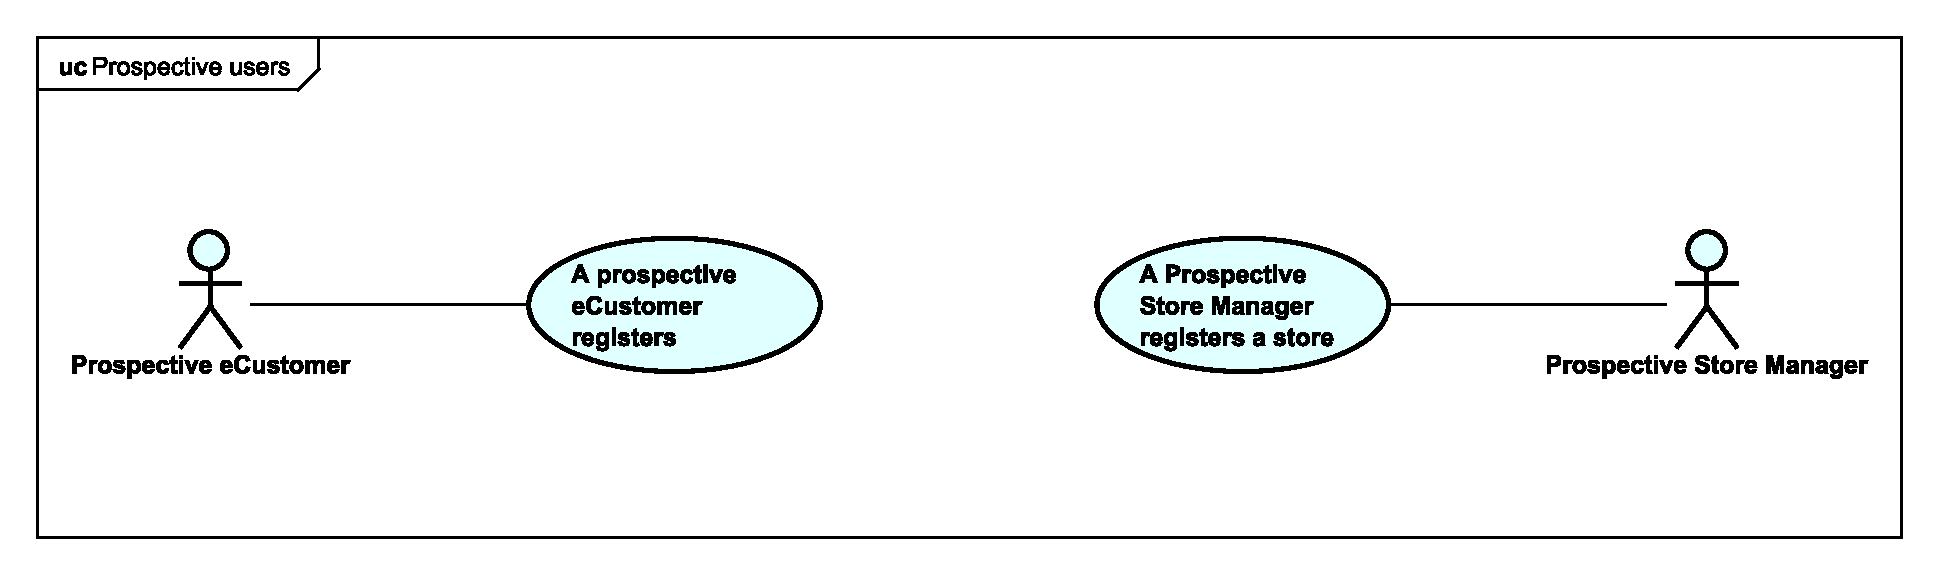
\includegraphics[width=\linewidth] {/use_cases/Prospective_users}
		\caption{Prospective users use cases}
		\label{prospective} }
	{	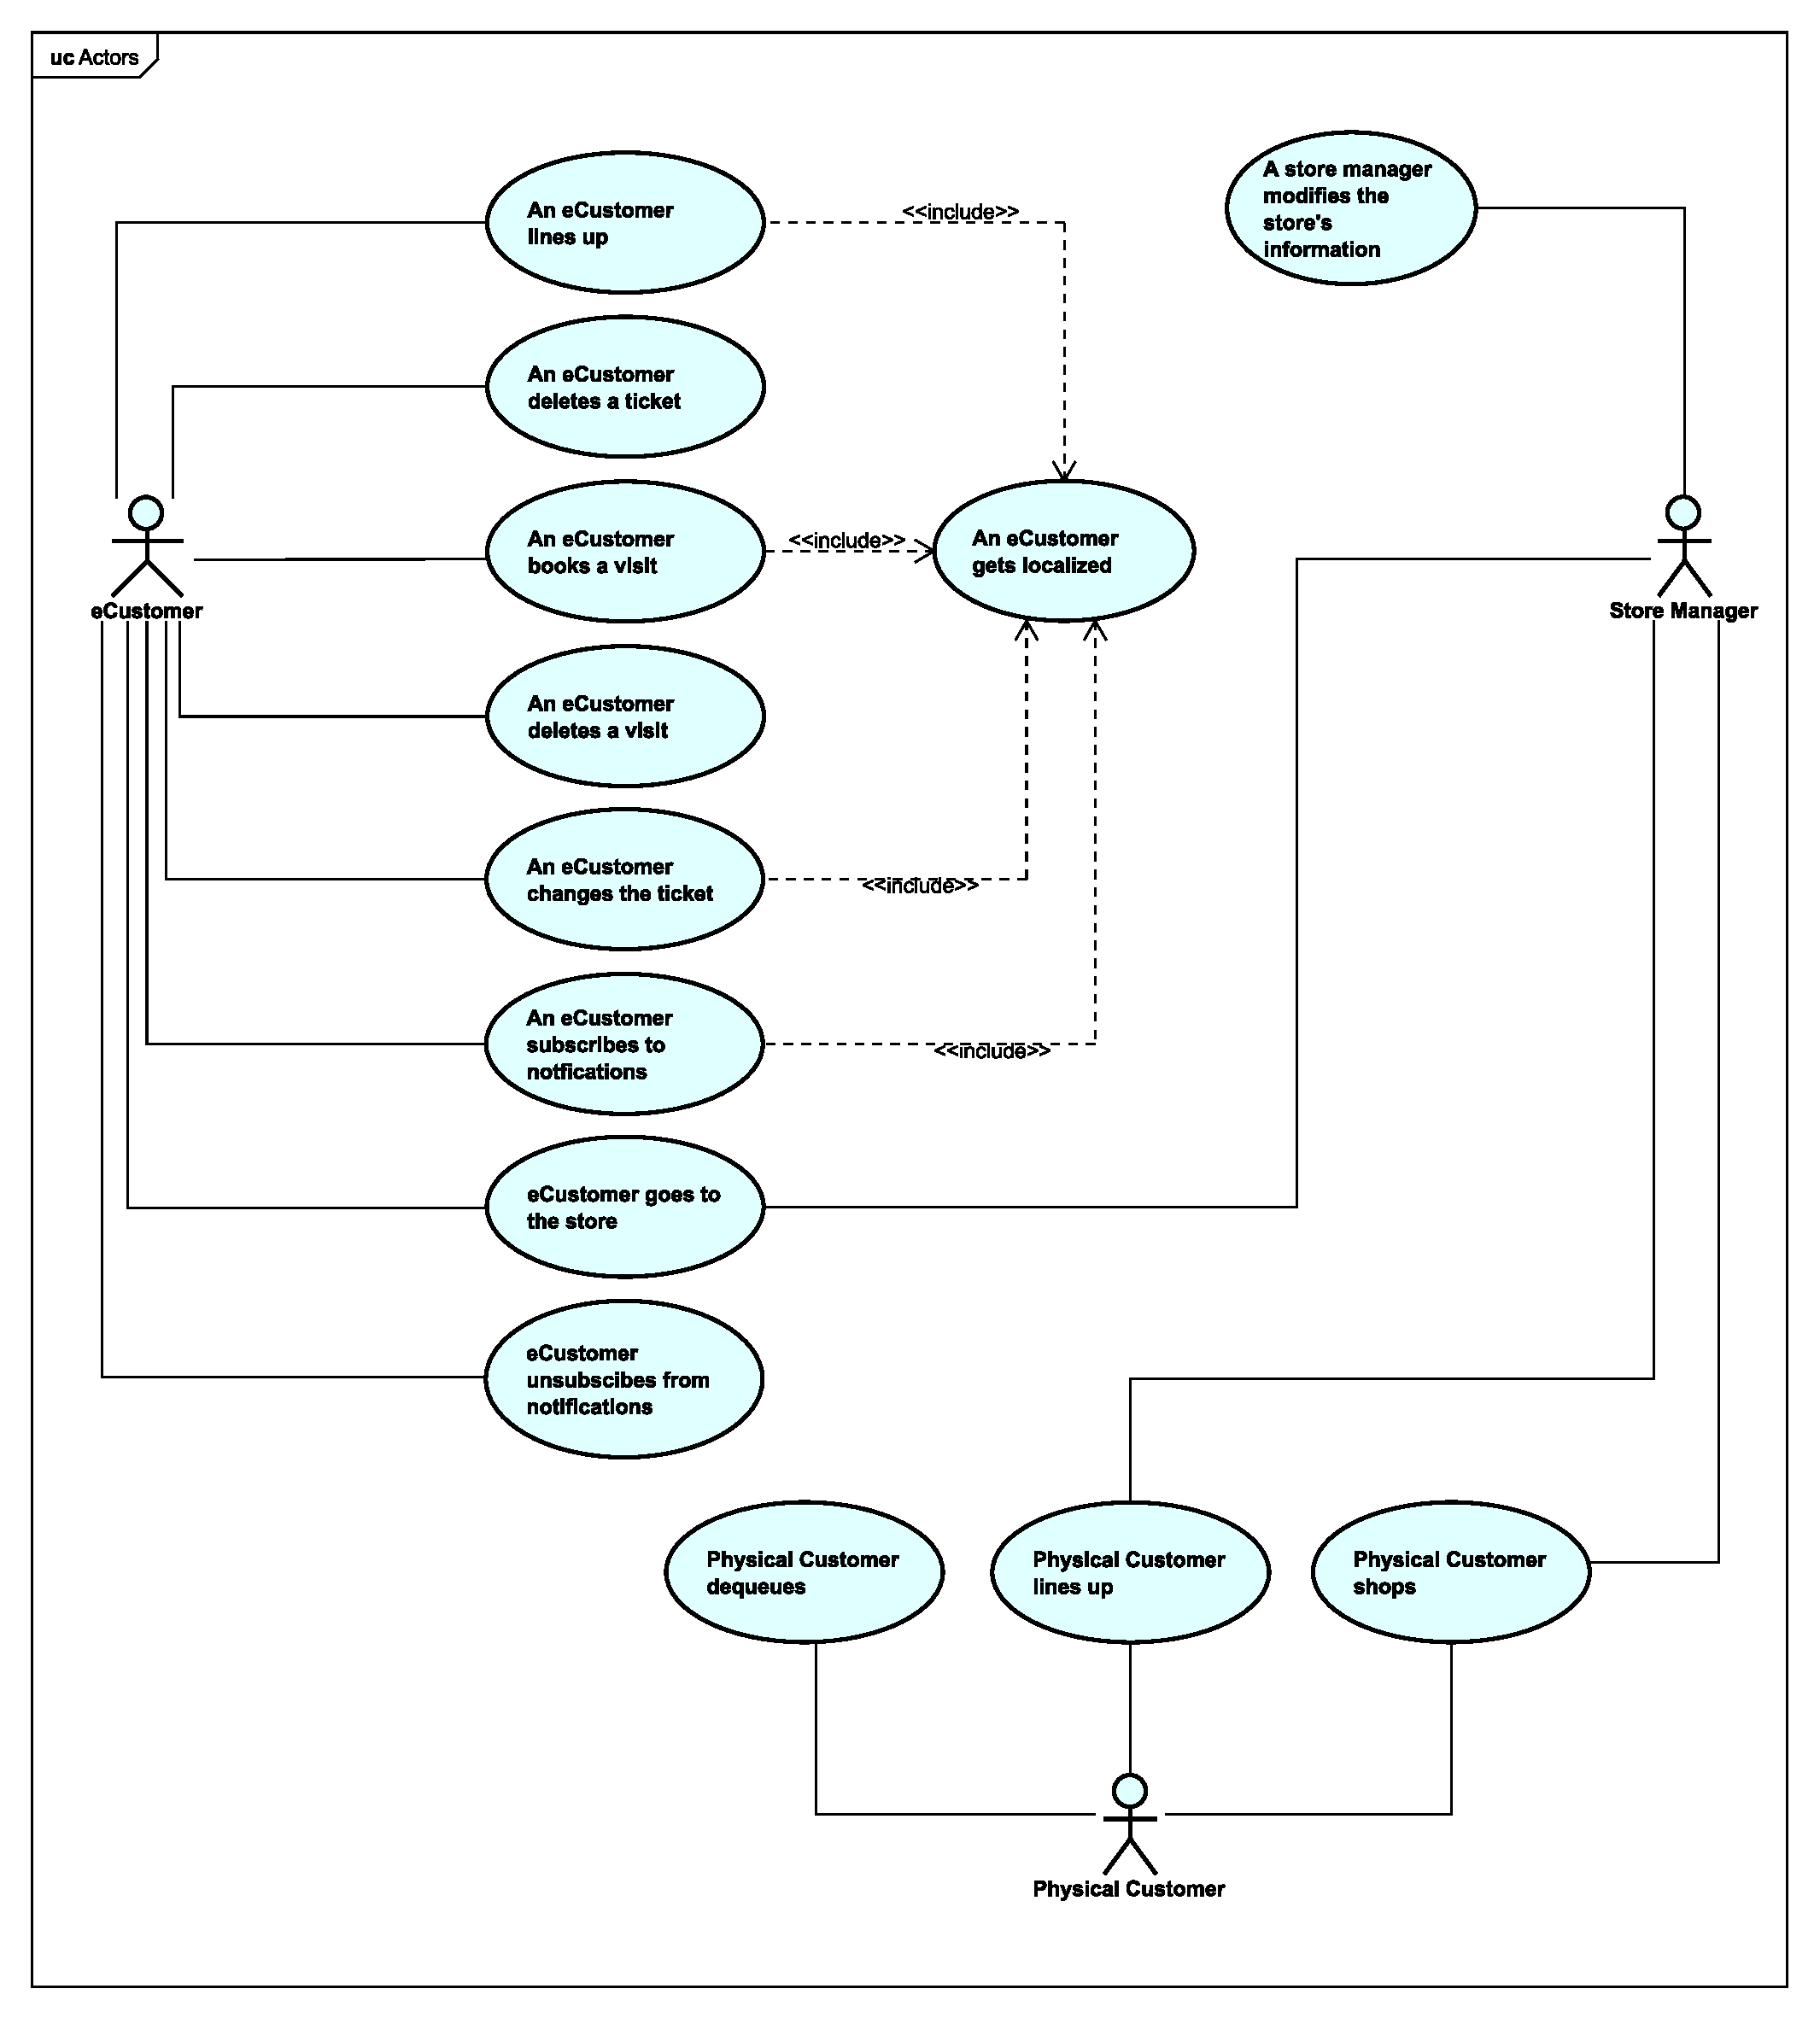
\includegraphics[width=\linewidth] {/use_cases/Actors}
		\caption{Actors use cases}
		\label{uc_actors} }
\end{figure}
\clearpage

% Sequence diagram file, to be included in requirements.tex

\subsection{Sequence diagrams}
Some sequence diagrams:

\begin{figure}[h]
	\centering	
	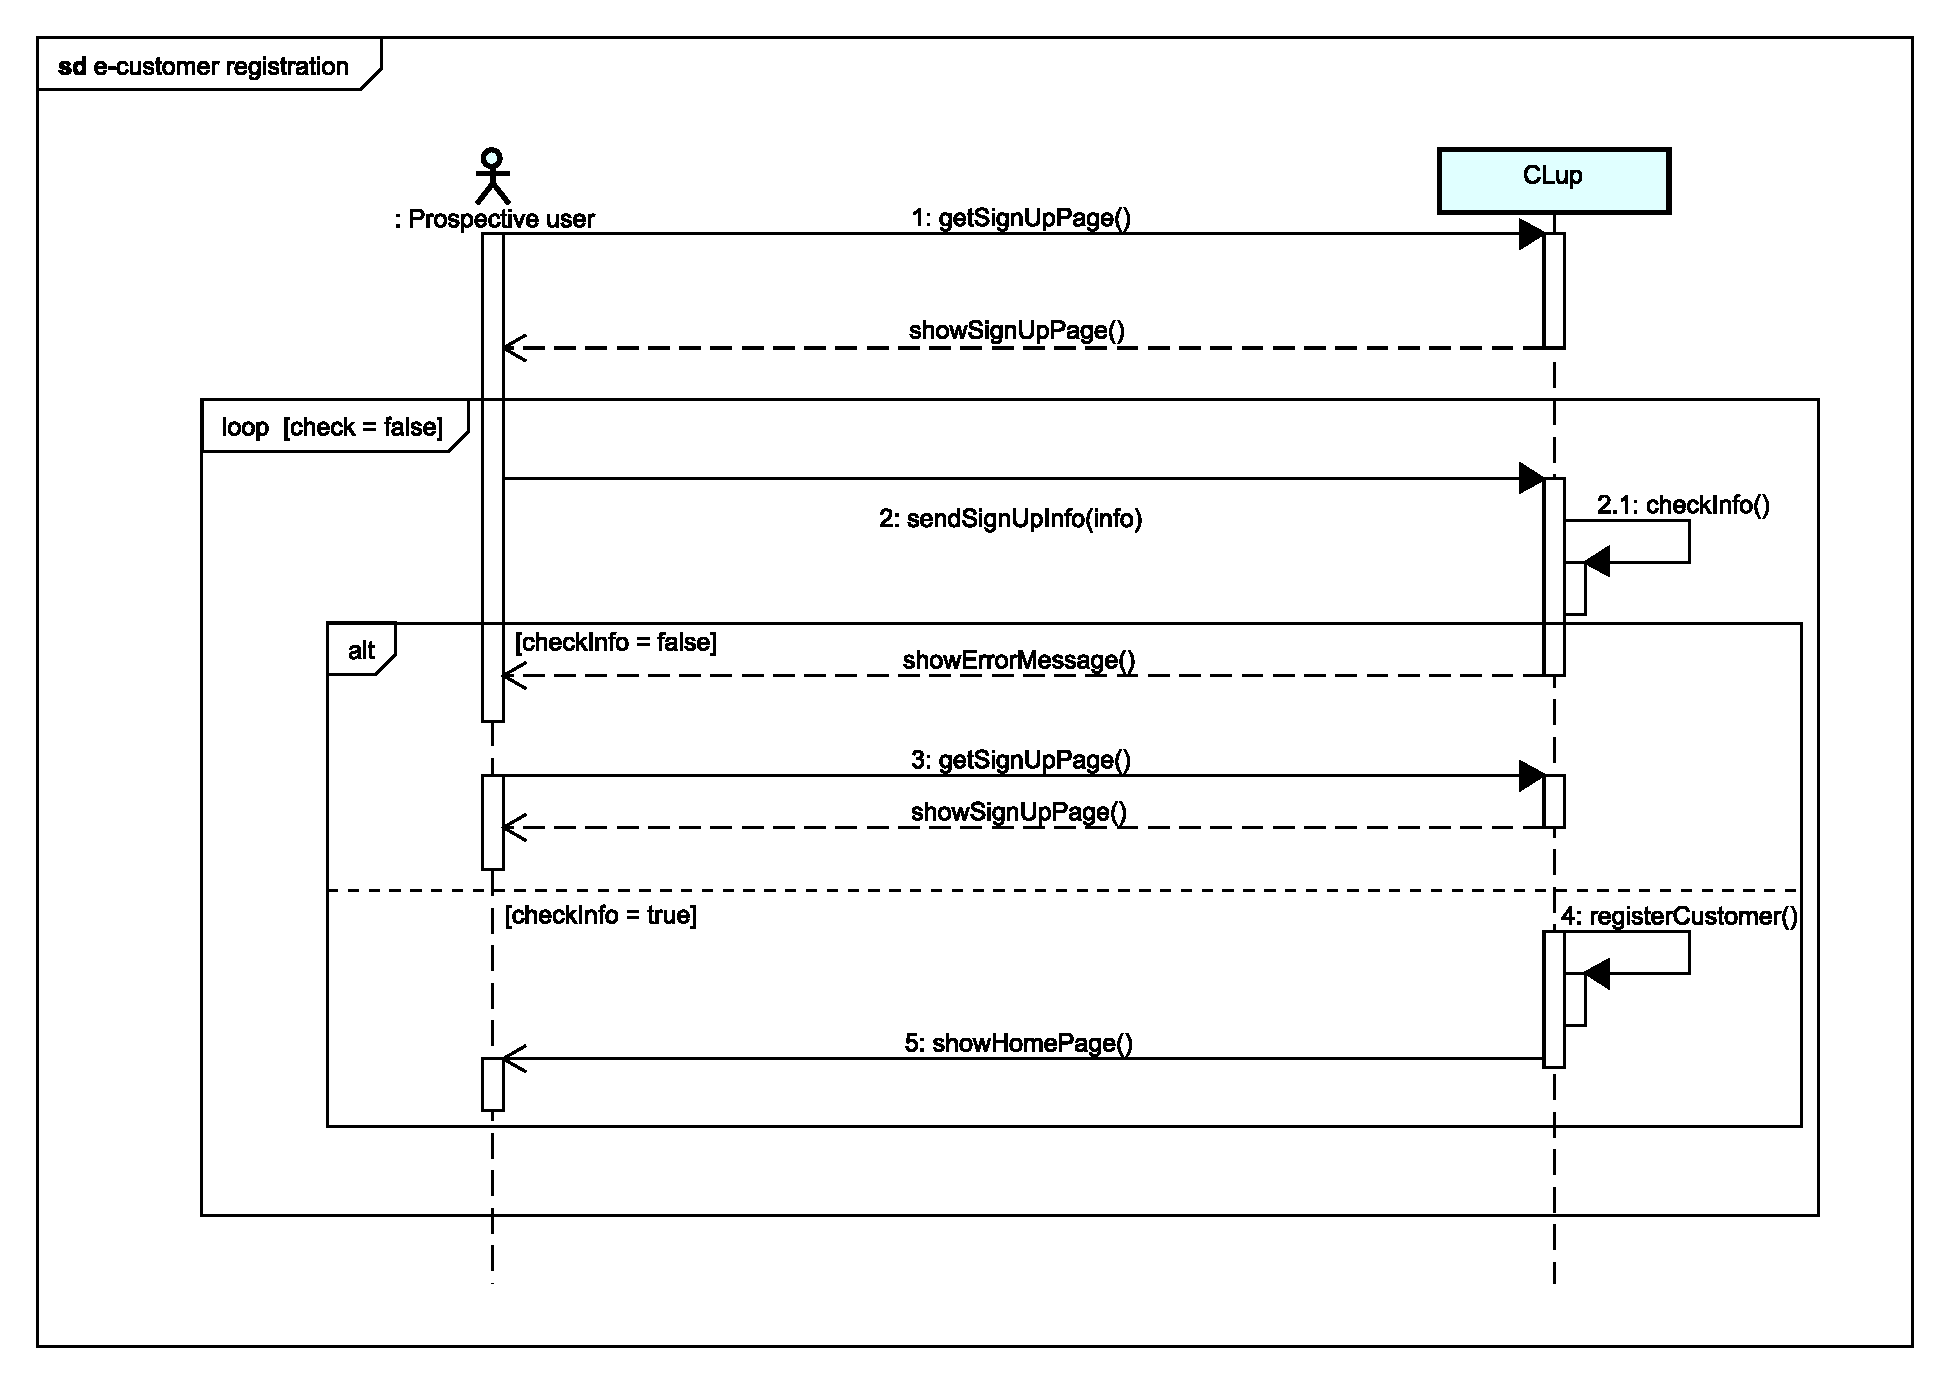
\includegraphics[width=\linewidth] {sequence_diagrams/e-customer_registration}
	\caption{e-Customer registration}
	\label{ec_reg} 
\end{figure}
\clearpage
\begin{figure}[h]
	\centering	
	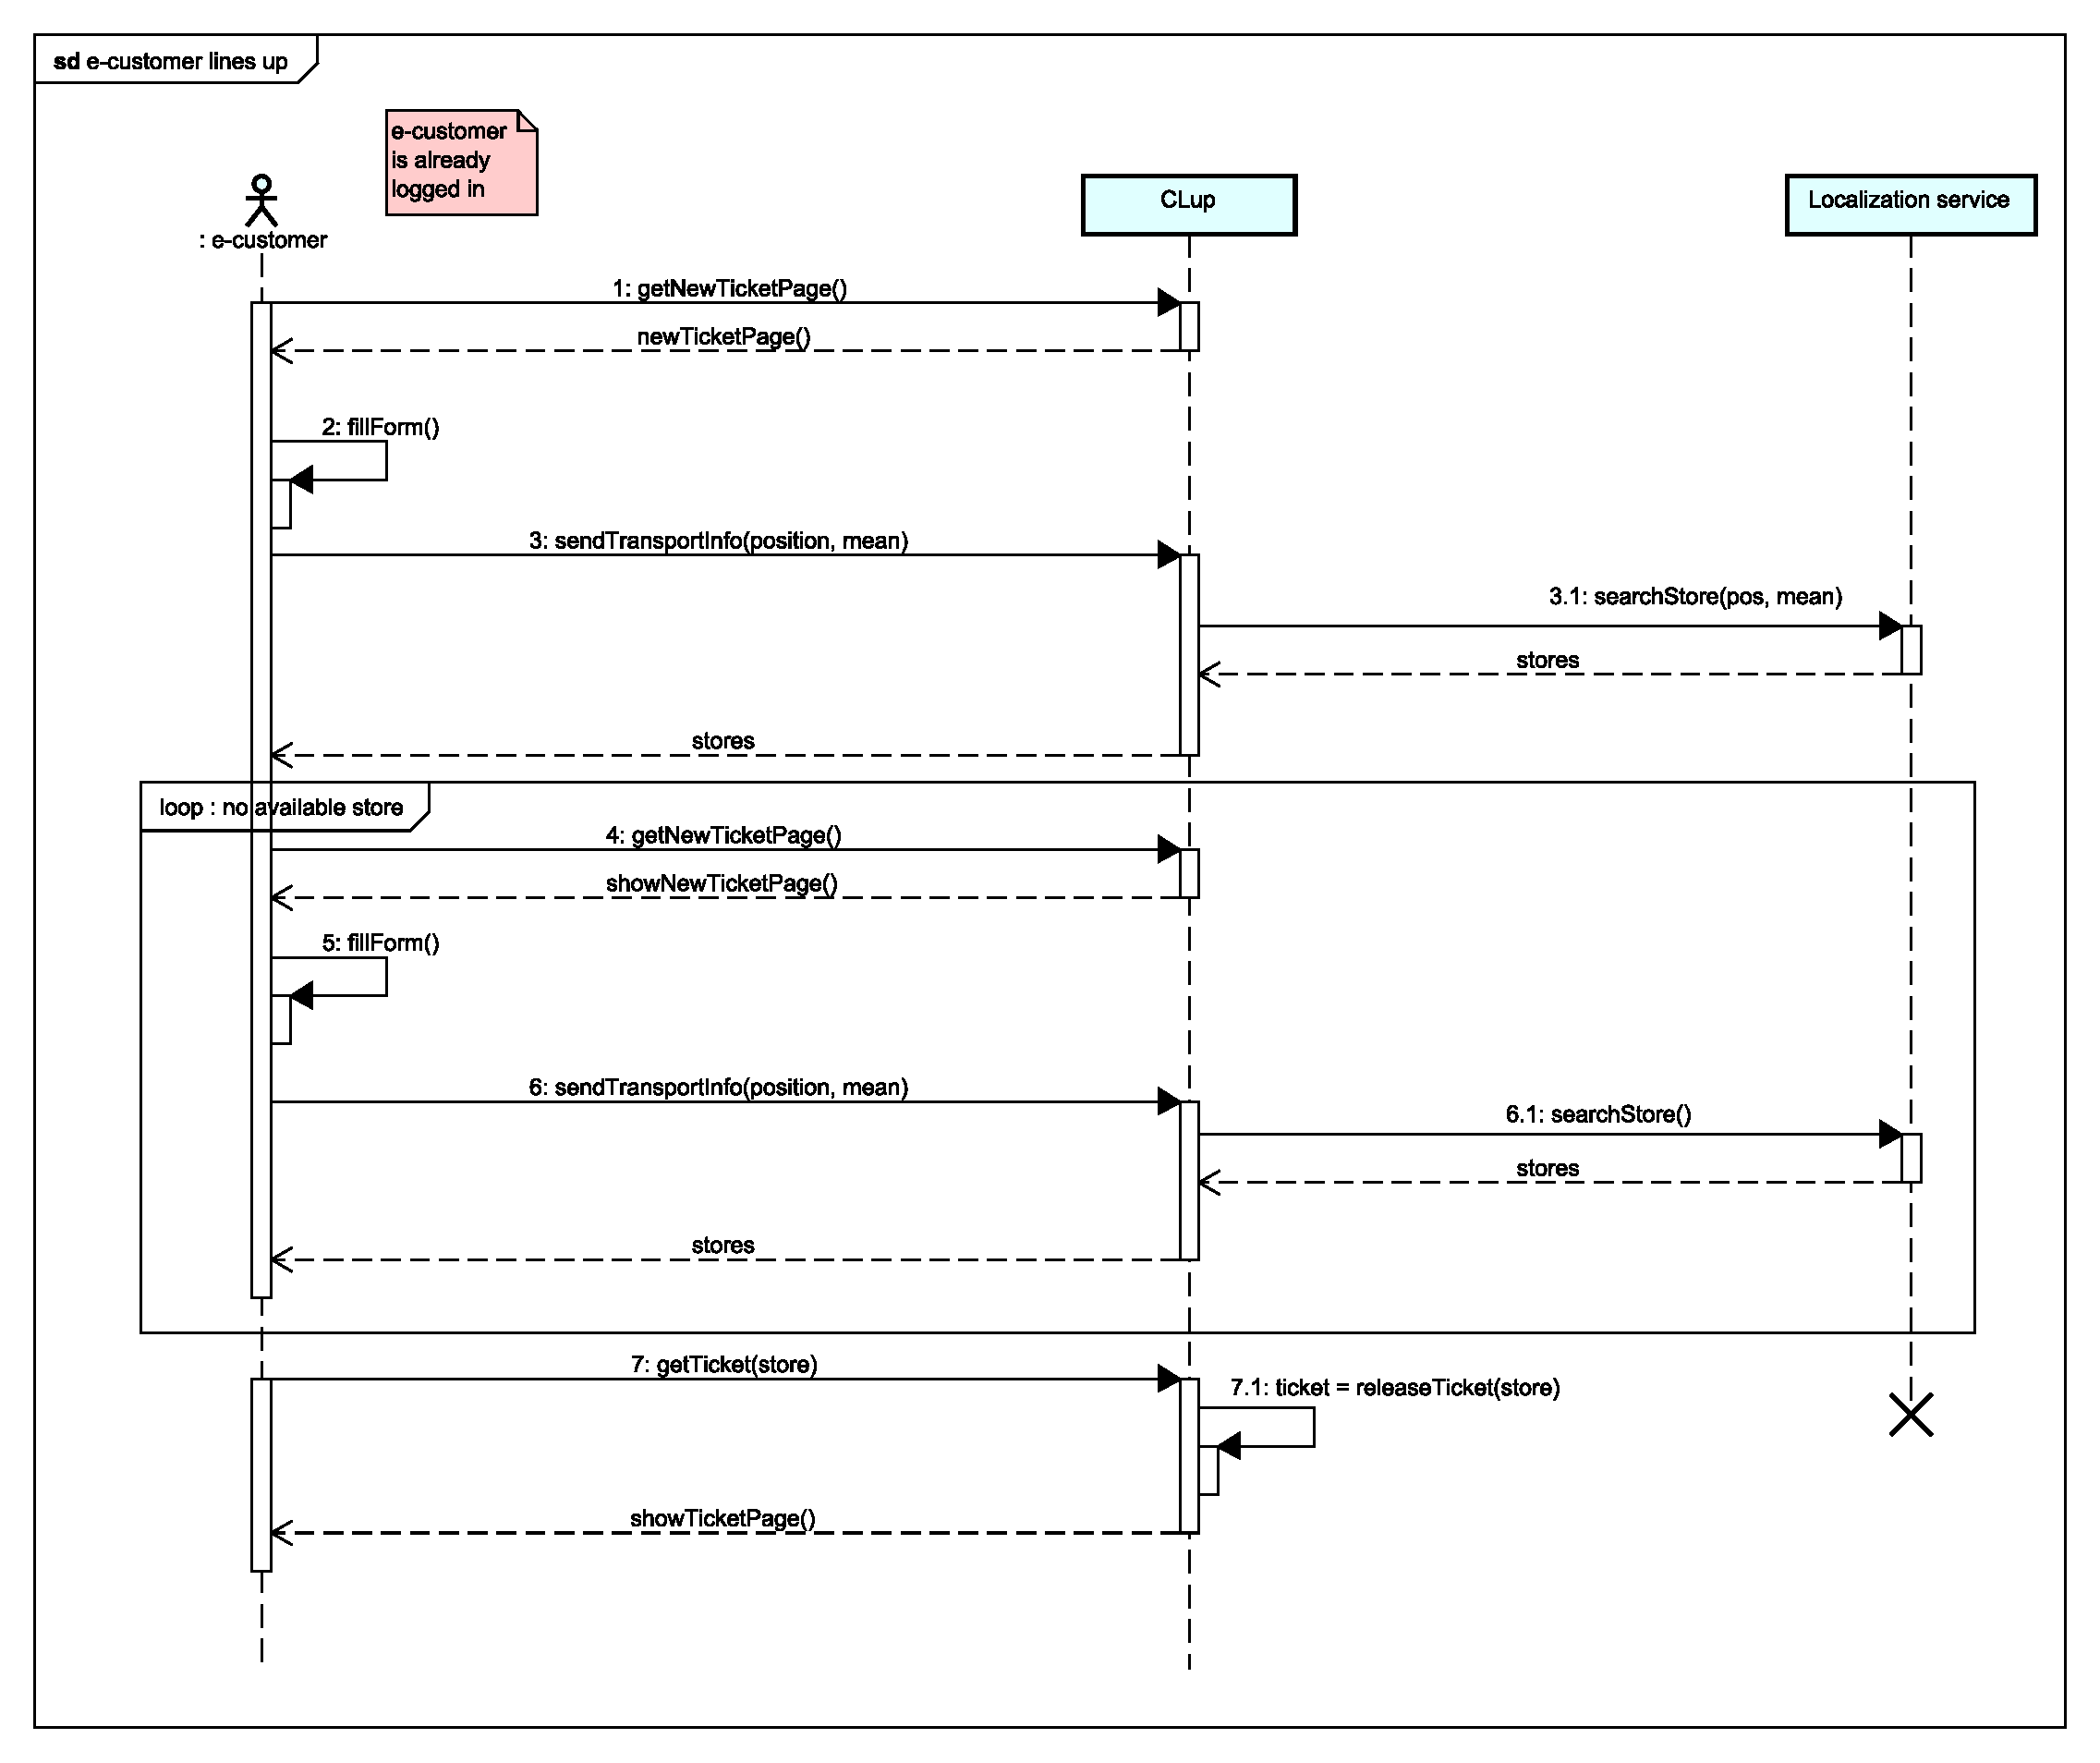
\includegraphics[width=\linewidth] {sequence_diagrams/e-customer_lines_up}
	\caption{e-Customer lines up}
	\label{ec_lup} 
\end{figure}
\clearpage
\begin{figure}[h]
	\centering	
	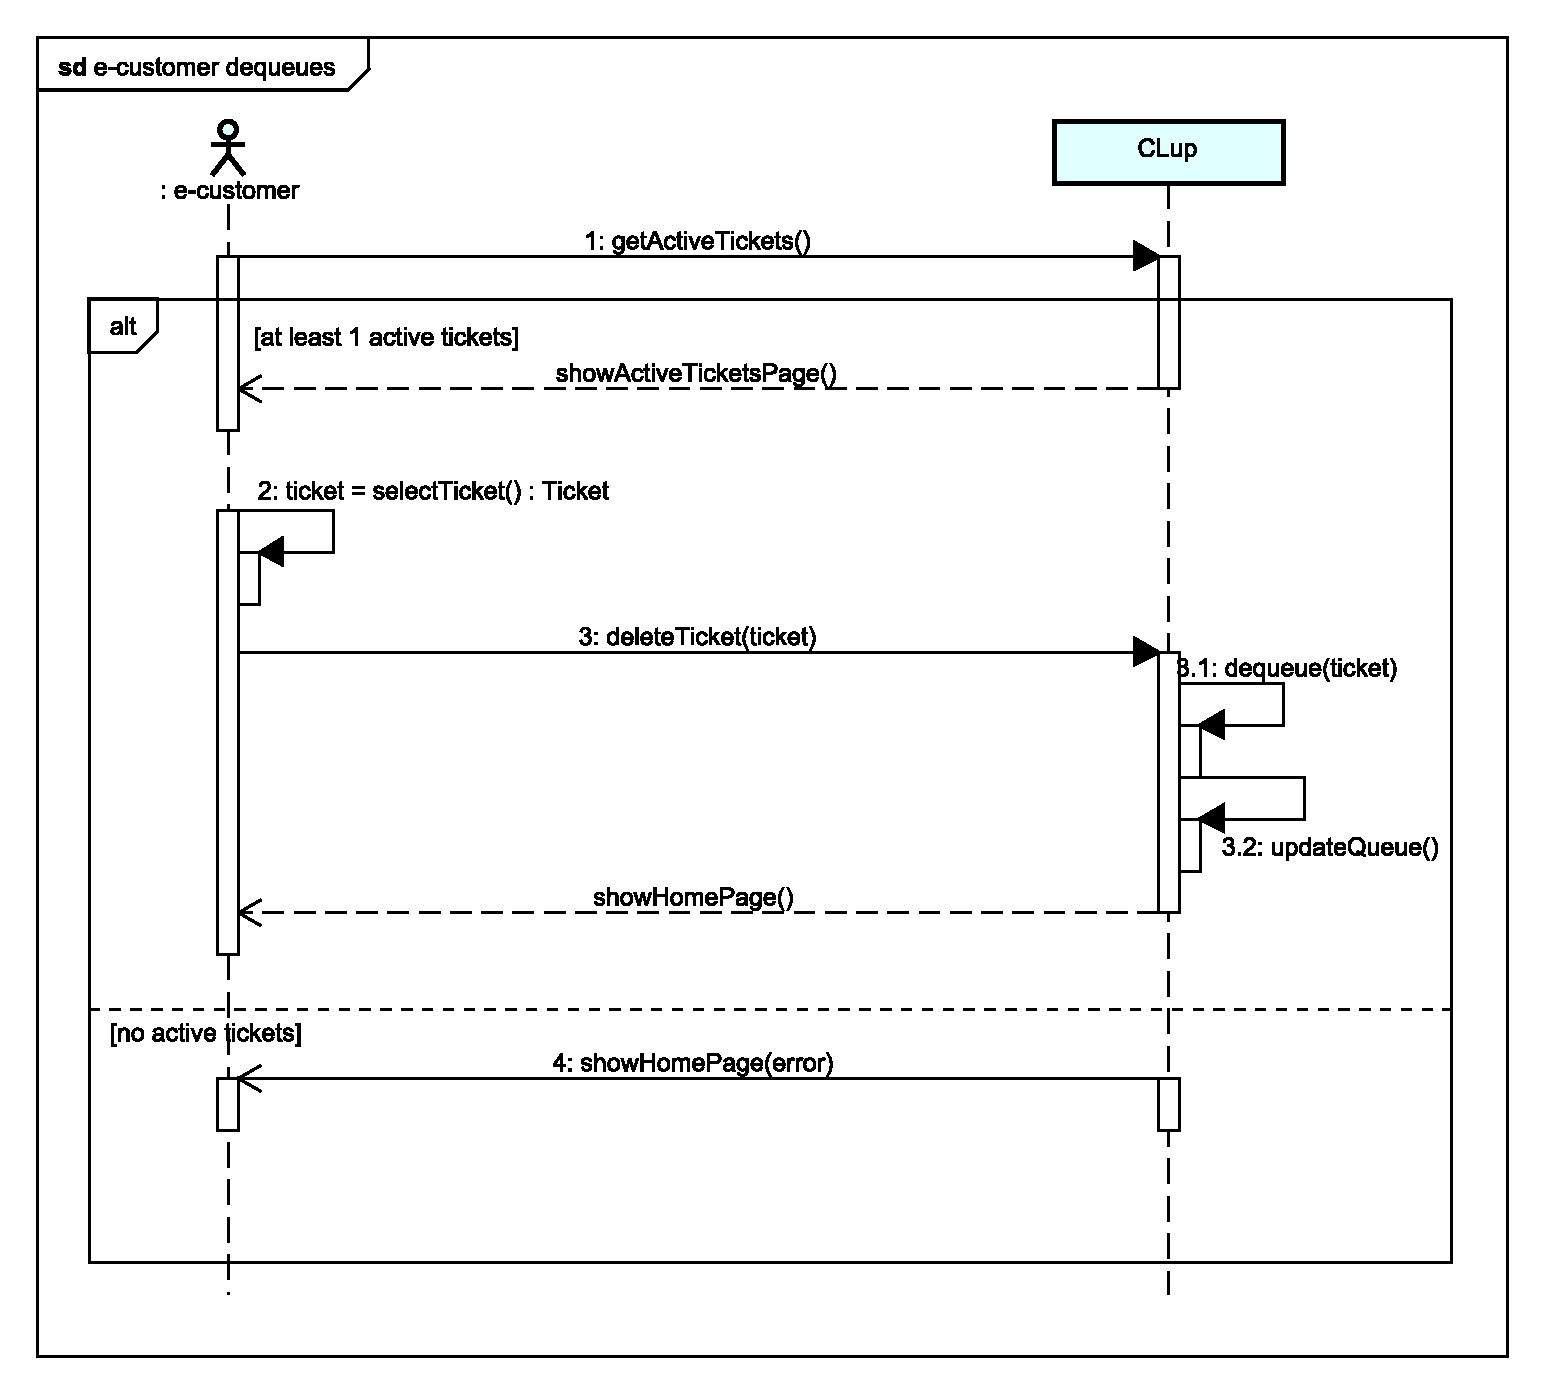
\includegraphics[width=\linewidth] {sequence_diagrams/e-customer_dequeues}
	\caption{e-Customer dequeues}
	\label{ec_deq} 
\end{figure}
\clearpage
\begin{figure}[h]
	\centering	
	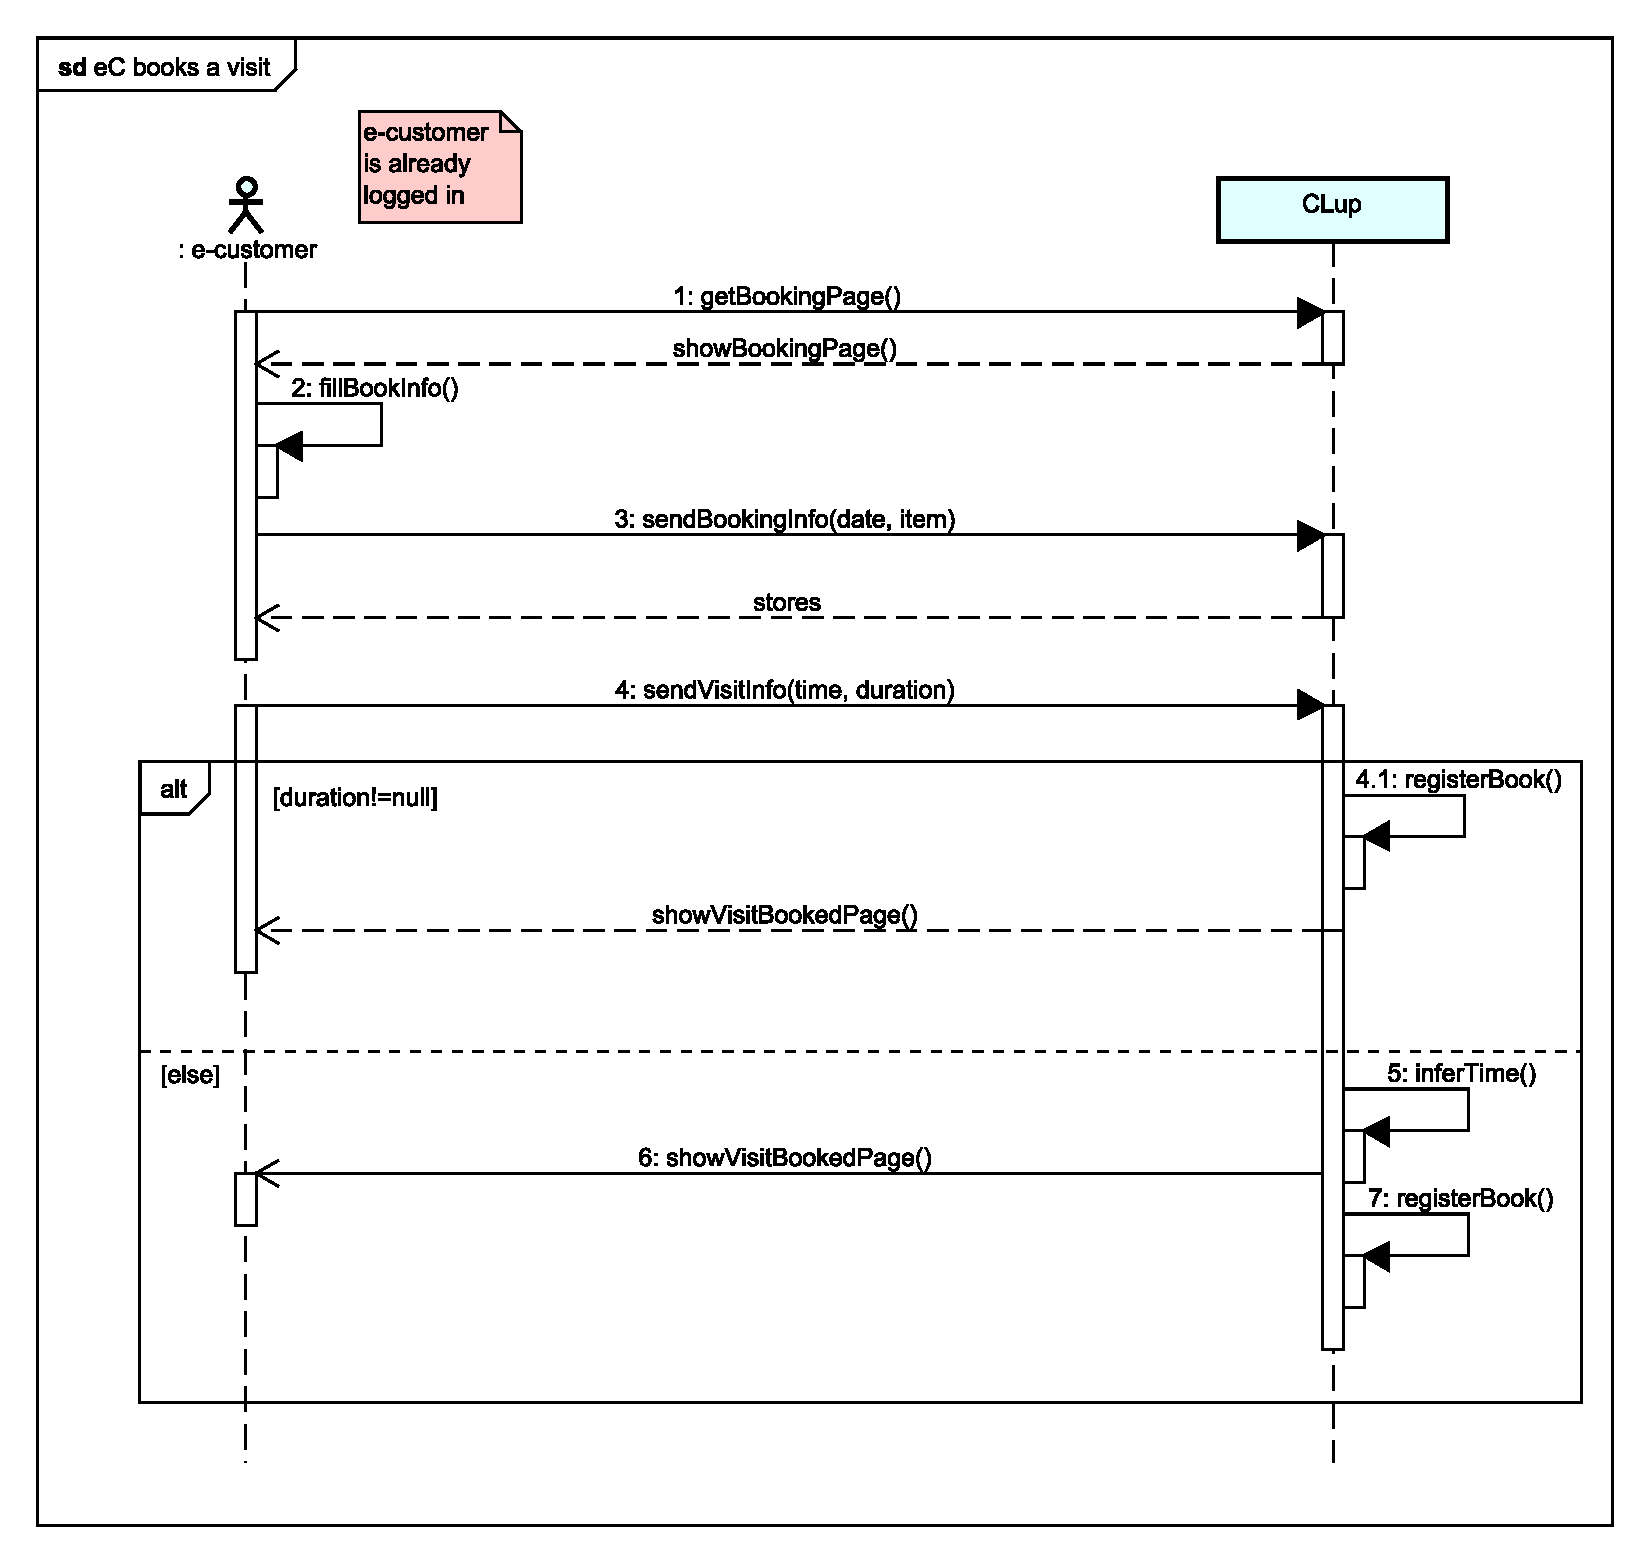
\includegraphics[width=\linewidth] {sequence_diagrams/eC_books_a_visit}
	\caption{e-Customer books a visit}
	\label{ec_book} 
\end{figure}
\clearpage
\begin{figure}[h]
	\centering	
	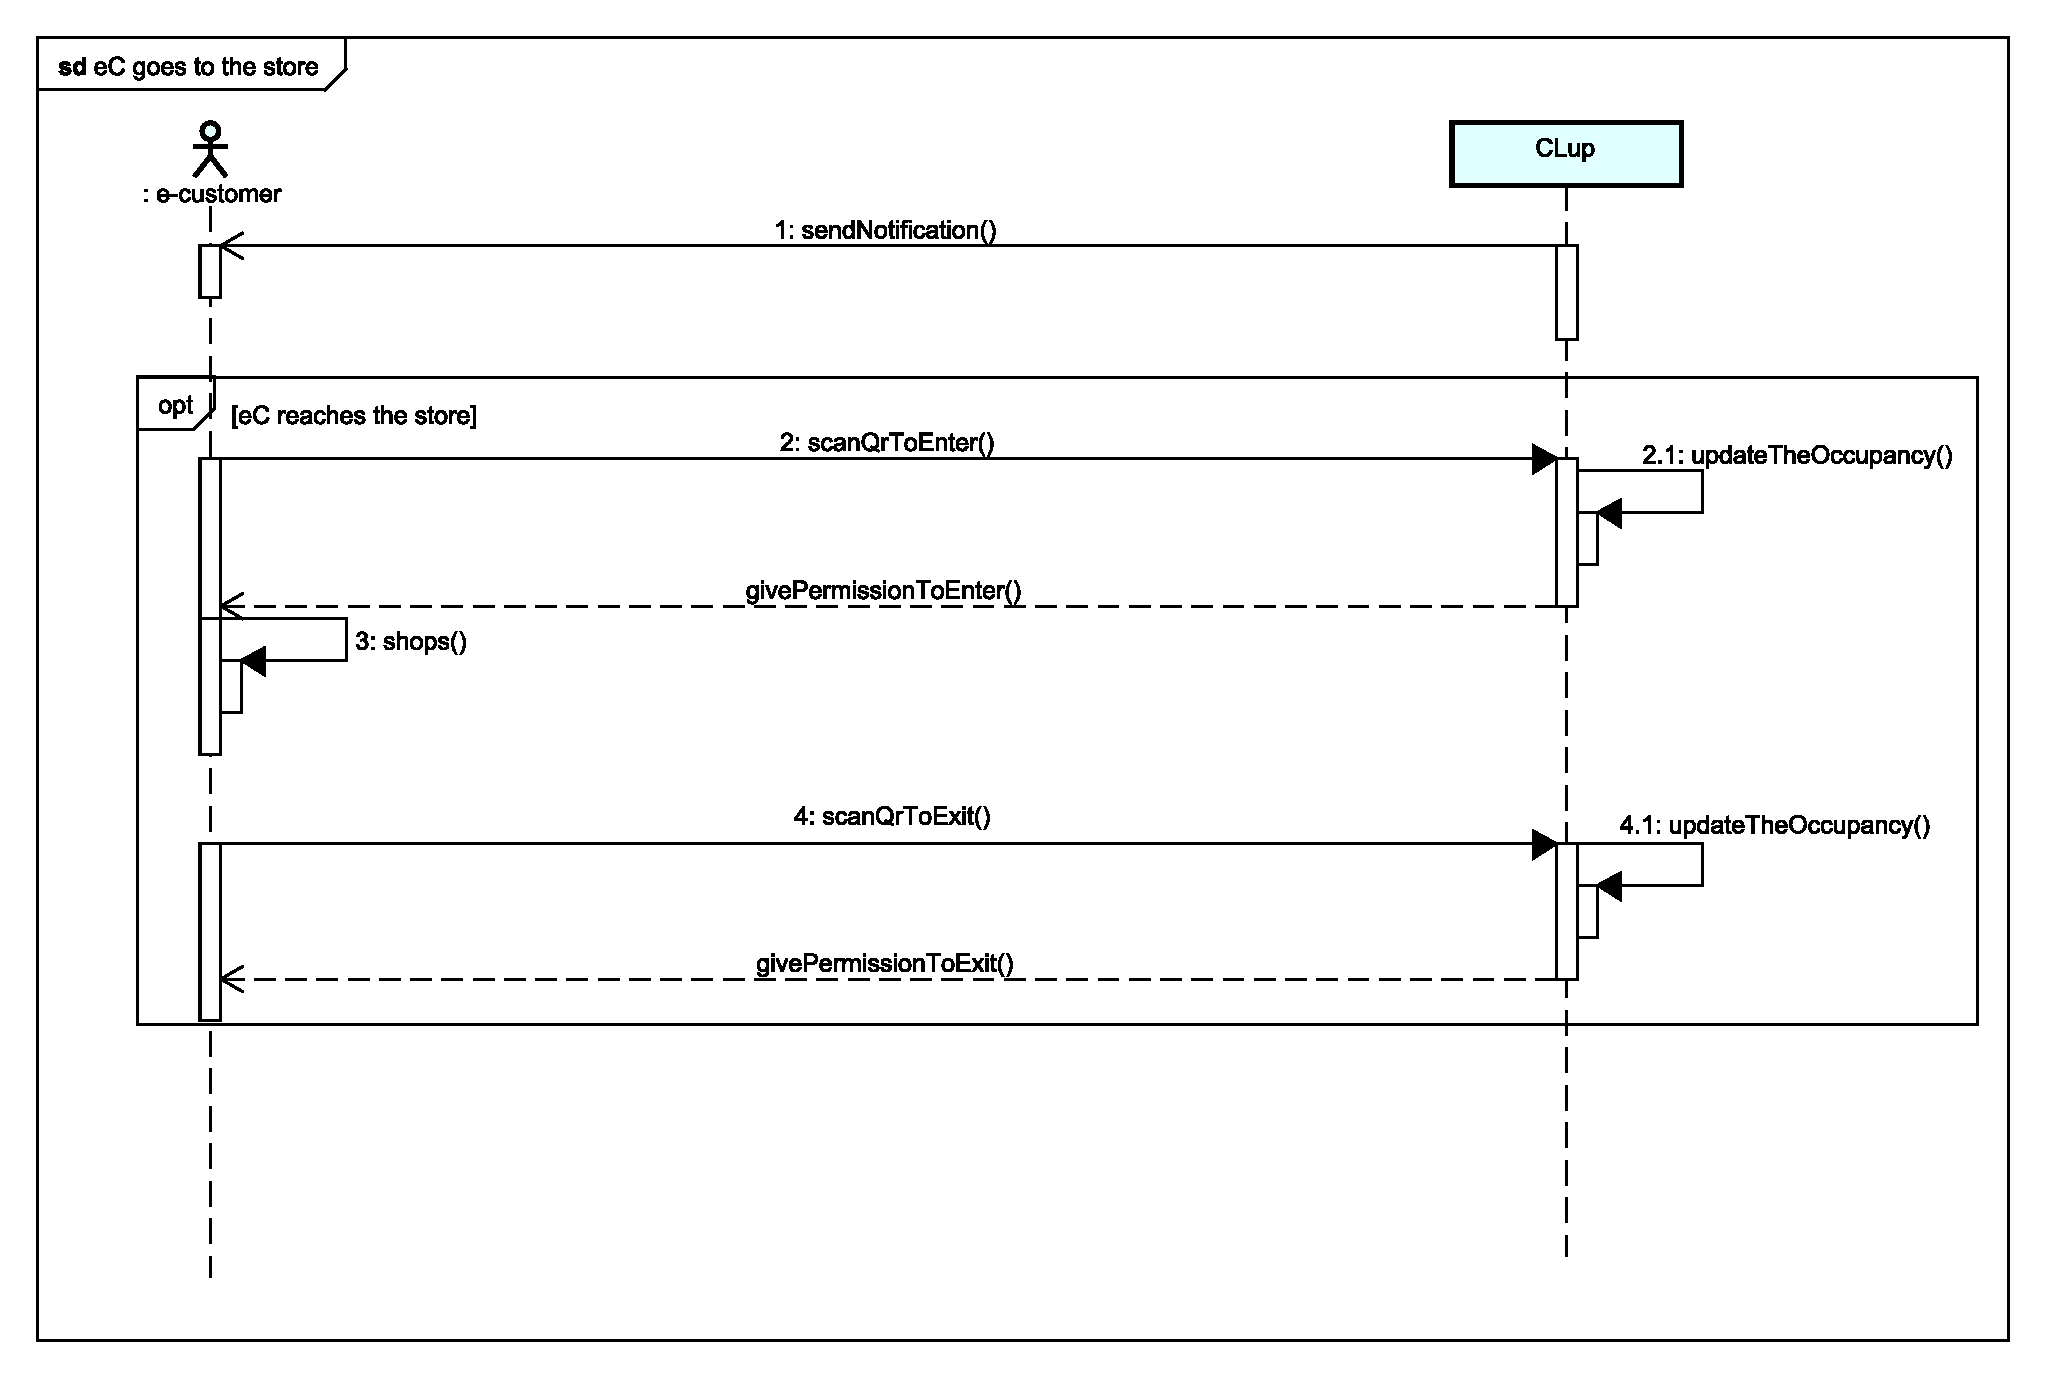
\includegraphics[width=\linewidth] {sequence_diagrams/eC_goes_to_the_store}
	\caption{e-Customer goes to the store}
	\label{ec_store} 
\end{figure}


% Goal, requirements and domains mapping. To be included in requirements.tex

\subsection{Goal Mapping}
In this section, goals are mapped to requirements and domain assumptions.

\subsubsection{[G0] Allow prospective e-Customers to register to the application}
\begin{itemize}
	\setlength\itemsep{-1mm}
	\item [\textbf{[R0]}] Must allow users to provide credentials
	\item [\textbf{[R1]}] Username must be unique 
	\\
	\item [\textbf{[D0]}] Prospective users will complete the registration process
	\item [\textbf{[D3]}] Information provided by users upon registration is correct
	\item [\textbf{[D11]}] The internet connection is always working
\end{itemize}

\subsubsection{[G1] Allow Prospective Store Managers to register to the application by adding their store}
\begin{itemize}
	\setlength\itemsep{-1mm}
	\item [\textbf{[R0]}] Must allow users to provide credentials
	\item [\textbf{[R1]}] Username must be unique 
	\item [\textbf{[R2]}] Store id must be unique
	\item [\textbf{[R3]}] Must allow store managers to add or modify their store’s information
	\\
	\item [\textbf{[D0]}] Prospective users will complete the registration process
	\item [\textbf{[D3]}] Information provided by users upon registration is correct
	\item [\textbf{[D7]}] Information about stores inserted by SMs is correct
	\item [\textbf{[D11]}] The internet connection is always working
\end{itemize}

\subsubsection{[G2] Allow e-customers to line up from home}
\begin{itemize}
	\setlength\itemsep{-1mm}
	\item [\textbf{[R4]}] Users must be able to login
	\item [\textbf{[R5]}] Must be able to provide the list of available stores in the user’s proximity
	\item [\textbf{[R6]}] Must know the e-Customer’s position
	\begin{itemize}[itemsep=-1mm, topsep=-1mm]
		\item [\textbf{[R6.1]}] Must localize the e-Customer or let them provide manually a position
	\end{itemize}
	\item [\textbf{[R7]}] Must assign a unique and sequential reservation id
	\item [\textbf{[R8]}] Must generate a QR code to be scanned at entrance and exit
	\item [\textbf{[R9]}] Must let e-Customers choose their mean of transport
	\item [\textbf{[R10]}] Must allow the entrance when it is the customer’s turn
	\item [\textbf{[R11]}] Must allow a delay of at most M minutes on a customer’s turn
	\item [\textbf{[R12]}] Must show e-Customers the number of enqueued customers in front of them
	\item [\textbf{[R13]}] Must show users historical data on given weekdays
	\item [\textbf{[R14]}] At least P% places must be reserved for tickets
	\item [\textbf{[R15]}] Must notify e-Customers within a suitable time from entrance
	\begin{itemize}[itemsep=-1mm, topsep=-1mm]
		\item [\textbf{[R15.1]}] Notification time must be based on current store occupation 
		\item [\textbf{[R15.2]}] Notification time must be based on estimated travel time
	\end{itemize}
	\item [\textbf{[R16]}] Must let e-Customers advance if a preceding customer dequeued
	\\
	\item [\textbf{[D1]}] Only people enqueued access the stores (both app and physical)
	\item [\textbf{[D2]}] Information provided by e-customers corresponds to their will
	\item [\textbf{[D4]}] Customers enter only if allowed by the application
	\item [\textbf{[D5]}] Customers respect the choices made during the input phase
	\item [\textbf{[D6]}] Calculated travel time is correct
	\item [\textbf{[D7]}] Information about stores inserted by SMs is correct
	\item [\textbf{[D8]}] Customers entering a store exit after some time
	\item [\textbf{[D9]}] If a client exits at a given time, he must have entered in the same opening period
	\item [\textbf{[D10]}] Ticket printers and QR readers work properly
	\item [\textbf{[D11]}] The internet connection is always working
	\item [\textbf{[D12]}] Users accept to receive notifications from the application
	\item [\textbf{[D13]}] Stores show the current customer number
	\item [\textbf{[D14]}] The external web mapping system is always available and there is signal
\end{itemize}

\subsubsection{[G2.1] Allow e-Customers to dequeue}
\begin{itemize}
	\setlength\itemsep{-1mm}
	\item [\textbf{[R4]}] Users must be able to login
	\\
	\item [\textbf{[D11]}] The internet connection is always working
\end{itemize}

\subsubsection{[G3] Allow Store Managers to monitor entrances}
\begin{itemize}
	\setlength\itemsep{-1mm}
	\item [\textbf{[R3]}] Must allow store managers to add or modify their store’s information
	\item [\textbf{[R4]}] Users must be able to login
	\item [\textbf{[R17]}] Must keep track of people inside the stores
	\begin{itemize}[itemsep=-1mm, topsep=-1mm]
		\item [\textbf{[R17.1]}] Must allow scanning QR codes on entrance and exit
	\end{itemize}
	\item [\textbf{[R18]}] Must not allow the entrance of more customers than prescribed
	\\
	\item [\textbf{[D1]}] Only people enqueued access the stores (both app and physical)
	\item [\textbf{[D4]}] Customers enter only if allowed by the application
	\item [\textbf{[D5]}] Customers respect the choices made during the input phase
	\item [\textbf{[D7]}] Information about stores inserted by SMs is correct
	\item [\textbf{[D8]}] Customers entering a store exit after some time
	\item [\textbf{[D9]}] If a client exits at a given time, he must have entered in the same opening period
	\item [\textbf{[D10]}] Ticket printers and QR readers work properly
	\item [\textbf{[D11]}] The internet connection is always working
	\item [\textbf{[D13]}] Stores show the current customer number
\end{itemize}

\subsubsection{[G4] Allow customers to physically line up}
\begin{itemize}
	\setlength\itemsep{-1mm}
	\item [\textbf{[R7]}] Must assign a unique and sequential reservation id
	\item [\textbf{[R8]}] Must generate a QR code to be scanned at entrance and exit
	\item [\textbf{[R10]}] Must allow the entrance when it is the customer’s turn
	\item [\textbf{[R11]}] Must allow a delay of at most M minutes on a customer’s turn
	\item [\textbf{[R20]}] Physical tickets must be placed on the same queue as virtual ones
	\item [\textbf{[R21]}] Physical tickets must be printed
	\\
	\item [\textbf{[D1]}] Only people enqueued access the stores (both app and physical)
	\item [\textbf{[D4]}] Customers enter only if allowed by the application
	\item [\textbf{[D8]}] Customers entering a store exit after some time
	\item [\textbf{[D9]}] If a client exits at a given time, he must have entered in the same opening period
	\item [\textbf{[D10]}] Ticket printers and QR readers work properly
	\item [\textbf{[D11]}] The internet connection is always working
	\item [\textbf{[D13]}] Stores show the current customer number
\end{itemize}

\subsubsection{[G4.1] Allow Physical Customers to dequeue}
\begin{itemize}
	\setlength\itemsep{-1mm}
	\item [\textbf{[R11]}] Must allow a delay of at most M minutes on a customer’s turn
	\item [\textbf{[R22]}] Must allow Physical Customers to scan their code in order to dequeue
	\\
	\item [\textbf{[D10]}] Ticket printers and QR readers work properly
	\item [\textbf{[D11]}] The internet connection is always working
	\item [\textbf{[D13]}] Stores show the current customer number
\end{itemize}

\subsubsection{[G5] Allow e-Customers to book a visit}
\begin{itemize}
	\setlength\itemsep{-1mm}
	\item [\textbf{[R4]}] Users must be able to login
	\item [\textbf{[R5]}] Must be able to provide the list of available stores in the user’s proximity
	\item [\textbf{[R6]}] Must know the e-Customer’s position
	\begin{itemize}[itemsep=-1mm, topsep=-1mm]
		\item [\textbf{[R6.1]}] Must localize the e-Customer or let them provide manually a position
	\end{itemize}
	\item [\textbf{[R7]}] Must assign a unique and sequential reservation id
	\item [\textbf{[R8]}] Must generate a QR code to be scanned at entrance and exit
	\item [\textbf{[R9]}] Must let e-Customers choose their mean of transport
	\item [\textbf{[R10]}] Must allow the entrance when it is the customer’s turn
	\item [\textbf{[R11]}] Must allow a delay of at most M minutes on a customer’s turn
	\item [\textbf{[R13]}] Must show users historical data on given weekdays
	\item [\textbf{[R14]}] At least P\% places must be reserved for tickets
	\item [\textbf{[R15]}] Must notify e-Customers within a suitable time from entrance
	\begin{itemize}[itemsep=-1mm, topsep=-1mm]
		\item [\textbf{[R15.2]}] Notification time must be based on estimated travel time
	\end{itemize}
	\item [\textbf{[R23]}] e-Customers who book a visit must be allowed to enter at their chosen time
	\item [\textbf{[R24]}] Must let e-Customers insert the expected duration of the visit
	\begin{itemize}[itemsep=-1mm, topsep=-1mm]
		\item [\textbf{[R24.1]}] Must be able to infer and suggest the duration for long term customers
	\end{itemize}
	\item [\textbf{[R25]}] Must let e-Customers insert a list of items/categories they intend to buy
	\\
	\item [\textbf{[D1]}] Only people enqueued access the stores (both app and physical)
	\item [\textbf{[D2]}] Information provided by e-customers corresponds to their will
	\item [\textbf{[D4]}] Customers enter only if allowed by the application
	\item [\textbf{[D5]}] Customers respect the choices made during the input phase
	\item [\textbf{[D6]}] Calculated travel time is correct
	\item [\textbf{[D7]}] Information about stores inserted by SMs is correct
	\item [\textbf{[D8]}] Customers entering a store exit after some time
	\item [\textbf{[D10]}] Ticket printers and QR readers work properly
	\item [\textbf{[D11]}] The internet connection is always working
	\item [\textbf{[D12]}] Users accept to receive notifications from the application
	\item [\textbf{[D14]}] The external web mapping system is always available and there is signal
\end{itemize}

\subsubsection{[G5.1] Allow e-Customers to delete a visit}
\begin{itemize}
	\setlength\itemsep{-1mm}
	\item [\textbf{[R4]}] Users must be able to login
	\\
	\item [\textbf{[D11]}] The internet connection is always working
\end{itemize}

\subsubsection{[G6] Can suggest alternative slots to balance the number of customers}
\begin{itemize}
	\setlength\itemsep{-1mm}
	\item [\textbf{[R4]}] Users must be able to login
	\item [\textbf{[R6]}] Must know the e-Customer’s position
	\begin{itemize}[itemsep=-1mm, topsep=-1mm]
		\item [\textbf{[R6.1]}] Must localize the e-Customer or let them provide manually a position
	\end{itemize}
	\item [\textbf{[R17]}] Must keep track of people inside the stores
	\item [\textbf{[R26]}] Alternatives must be based on information provided by the e-Customer and store occupation (both real time and historical)
	\\
	\item [\textbf{[D4]}] Customers enter only if allowed by the application
	\item [\textbf{[D5]}] Customers respect the choices made during the input phase
	\item [\textbf{[D6]}] Calculated travel time is correct
	\item [\textbf{[D7]}] Information about stores inserted by SMs is correct
	\item [\textbf{[D8]}] Customers entering a store exit after some time
	\item [\textbf{[D9]}] If a client exits at a given time, he must have entered in the same opening period
	\item [\textbf{[D11]}] The internet connection is always working
	\item [\textbf{[D14]}] The external web mapping system is always available and there is signal
\end{itemize}

\subsubsection{[G7] Allow e-Customers to manage slot notifications}
\begin{itemize}
	\setlength\itemsep{-1mm}
	\item [\textbf{[R4]}] Users must be able to login
	\item [\textbf{[R6]}] Must know the e-Customer’s position
	\begin{itemize}[itemsep=-1mm, topsep=-1mm]
		\item [\textbf{[R6.1]}] Must localize the e-Customer or let them provide manually a position
	\end{itemize}
	\item [\textbf{[R17]}] Must keep track of people inside the stores
	\item [\textbf{[R27]}] e-Customers must be able to subscribe to the notification service
	\item [\textbf{[R28]}] Must let e-Customers unsubscribe from the notification service
	\item [\textbf{[R29]}] The system must notify the e-Customers based on their choices
	\\
	\item [\textbf{[D2]}] Information provided by e-customers corresponds to their will
	\item [\textbf{[D7]}] Information about stores inserted by SMs is correct
	\item [\textbf{[D8]}] Customers entering a store exit after some time
	\item [\textbf{[D9]}] If a client exits at a given time, he must have entered in the same opening period
	\item [\textbf{[D11]}] The internet connection is always working
	\item [\textbf{[D12]}] Users accept to receive notifications from the application
	\item [\textbf{[D14]}] The external web mapping system is always available and there is signal
\end{itemize}

% Non-functional requirements page, to be included in requirements.tex

\subsection{Non-functional requirements}
An important non-functional requirement is the ease of use, given the wide variety of people potentially using the system. Requirements related to the system are as follows.

\subsubsection{Performance}
CLup, both for the app and the web application, should provide fast responses to user actions, possibly under 3 seconds\textsuperscript{\cite{speed}}. This result should account for about 150000 daily requests, based on competitor's data\textsuperscript{\cite{ufirst}}.

\subsubsection{Availability and reliability}
As a service used for primary needs connected to stores potentially open all day and every period of the year, CLup should be very robust and reliable, offering an availability of at least 0.999 (that corresponds to less than a day of downtime every year).

\subsubsection{Security}
All user information will need to be securely stored by the application. The communication between clients and server should be protected alongside QR codes, in order to ensure fairness in queue management too.

\subsubsection{Maintainability}
As in all software applications, maintainability should be a core property of CLup, enabling changes both related to modifications in functionalities and bug fixing.

\subsubsection{Portability}
The client system should be developed to be compatible with most of the mobile Operating Systems (for the mobile application) and browsers (for the web app). The latter option should prioritize mobile environments (i.e. smartphones, tablets) without precluding access to desktop-based systems, even if they are not the primary target of the application.

% Design constraints page, to be included in requirements.tex

\subsection{Design constraints}

\subsubsection{Hardware and software limitations}
The hardware and software requirements are stated here, divided by usage:
\begin{itemize}[itemsep=-1mm, topsep=-1mm]
	\item For the mobile application: 
	\begin{itemize}[itemsep=-1mm, topsep=-1mm]
		\item Operating system: Android 6.0+ or iOS 9+
		\item The device must be internet enabled
	\end{itemize}
	
	\item For the web application, a device with either:
	\begin{itemize}[itemsep=-1mm, topsep=-1mm]
		\item Mozilla Firefox 19.0+
		\item Google Chrome 25.0+
		\item Microsoft Edge 
		\item Safari 5.1+
		\item Opera 12.1+
	\end{itemize}
\end{itemize}	
A mobile device used by a Store Manager will also need a camera.

\subsubsection{Privacy policies}
The system will need to access some device data in order to function properly; the following table summarizes the permission requests:

\begin{center}
	\rowcolors{4}{white}{tablerow}
	\begin{tabular}{c | c | c | c | c }
		\multirow{2}{*}{Permission} & \multicolumn{2}{c|}{e-Customer} & \multicolumn{2}{c}{Store Manager} \\ \cline{2-5}
		                            & Mobile & Web                    & Mobile & Web                      \\ \hline
		          Storage           & Mandatory      &                       &       &  \\
		          Camera &  &  & Mandatory & Mandatory \\
		          Localization & Optional & Optional &  & 
	\end{tabular}
\end{center}

Moreover, in order to comply with privacy regulations\textsuperscript{\cite{gdpr}}, CLup:
\begin{itemize}[itemsep=-1mm, topsep=-1mm]
	\item Will ask for the user's consent for their data processing
	\item Will not use any of the user data for purposes different from the offered service
	\item Will not request personal data that is not necessary to offer the service
	\item Will not keep any personal data once it is not needed anymore
	\item Will ensure privacy and security by design
\end{itemize}



	
	% Alloy section
	\clearpage
	% Alloy section, to be included in RASD.tex

\section{Formal Analysis Using Alloy}
\label{sect:alloy}
This section describes the model defined through the Alloy language\textsuperscript{\cite{alloy}}. It is used to define the subset of the domain used to handle tickets, that represents the most critical portion of the system. 

As it can be noted in Section \ref{sect:run}, the chosen bitwidth is 7, thus allowing the generation of integers between $-64$ and $+63$ to meet all constraints.

% FIle to host alloy signatures, to be included in alloy.tex

\subsection{Signatures}
\begin{lstlisting}[language=alloy]
	// Ticket states
	enum State {
		ENQUEUED, 
		CANENTER, 
		DEQUEUED, 
		INSIDE, 
		COMPLETED, 
		WRONG
	}
	
	// All clients of stores
	sig Customer {
		tickets: set Ticket,
		visits: set Visit,
		insideStore: lone Store
	}
	
	// Store signature
	sig Store {
		capacity: one Int,
		delayWindow: one Int,
		queue: one Queue,
		inside: set Customer,
		hours: set OpeningHours
	} {
		capacity > 0
		delayWindow > 0
		#inside =< capacity 
	}
	
	// Signature containing sequences of tickets
	sig Queue {
		store: one Store,
		tickets: seq Ticket
	}
	
	// Ticket signature
	sig Ticket {
		nOrder: one Int,
		customer: one Customer,
		queue: one Queue,
		state: one State
	} {
		nOrder >= 0
	}
	
	// Signature representing a visit that occurred
	sig Visit {
		customer: one Customer,
		accessreq: one Ticket,
		store: one Store,
		weekday: one Int,
		datetimeIN: one DateTime,
		datetimeOUT: one DateTime
	} {
		weekday >= 1 and weekday =< 7
		accessreq.queue.store = store
		accessreq.customer = customer
		isBefore[datetimeIN.time, datetimeOUT.time]
		datetimeIN.time != datetimeOUT.time
	}
	
	// Stores' opening hours
	// In order to simplify the model, 
	// no store is open during day changes
	sig OpeningHours {
		weekday: one Int,
		openingTime: one Time,
		closingTime: one Time
	} {
		weekday > 0 and weekday =< 7
		isBefore[openingTime, closingTime]
		and (openingTime.hours != closingTime.hours 
			or openingTime.minutes != closingTime.minutes)
	}
	
	// Signature used to model time
	sig Time {
		hours: one Int,
		minutes: one Int
	} {
		hours >= 0 
		hours < 24 
		minutes >= 0 
		minutes < 60
	}
	
	// Signature to model a date 
	// (to simplify the year is assumed as 2020)
	sig Date {
		month: one Int,
		day: one Int
	} { 
		month >= 1 and month =< 12
		day >= 1
		(month = 4 or month = 6 or month = 9 or month = 11) 
			implies day =< 30
		else (month = 2) 
			implies day <= 29
		else day =< 31
	}
	
	// Union of date and time
	sig DateTime {
		date: one Date,
		time: one Time
	}
\end{lstlisting}
% Alloy facts, to be included in alloy.tex

\subsection{Facts}

\begin{lstlisting}[language=alloy]
	// Fact to define ticket unicity in queues
	fact uniqueTicketInQueue {
		// No different tickets having the same number
		no disj t, t': Ticket | all q: Queue |
			t in q.tickets.elems 
			and t' in q.tickets.elems
			and t.nOrder = t'.nOrder
		
		// No ticket is in a queue more than once
		all q: Queue | !q.tickets.hasDups
	}
	
	// Facts modeling necessary relations between signatures
	fact implications {
		// Customer <=> Ticket
		all c: Customer | all t: Ticket | 
			t in c.tickets iff t.customer = c
		
		// Customer <=> store
		all c: Customer | all s: Store | 
			s = c.insideStore iff c in s.inside
		
		// Queue <=> Store
		all q: Queue | all s: Store | 
			q.store = s iff s.queue = q
		
		// Queue => Ticket
		all t: Ticket | all q: Queue | 
			t in q.tickets.elems implies t.queue = q
		
		// Visit <=> Customer
		all v: Visit | all c: Customer |
			v.customer = c iff v in c.visits
	}

	// A ticket can correspond to at most one visit
	fact oneTicketPerVisit {
		no disj v,v': Visit | 
			v.accessreq = v'.accessreq
	}
	
	// A customer cannot request a ticket for a store 
	// they are already enqueued for
	fact noSameCustomerInQueue {
		all q: Queue | no disj t, t': Ticket |  
			t in q.tickets.elems 
			and t' in q.tickets.elems 
			and t.customer = t'.customer 
	}
	
	// A customer inside a store must have entered with a ticket
	fact customerInsideRequiresTicket {
		all c: Customer | all s: Store | c.insideStore = s implies 
			one t: Ticket | t.customer = c and t.state = INSIDE
	}
	
	// Ticket Ordering
	fact TicketOrder {
		all t: Ticket |
			t.nOrder = plus[t.queue.tickets.idxOf[t], 1]
	}
	
	// Ticket states
	fact ticketStates {
		all t: Ticket |  
		(!ticketInside[t] 
		and !ticketInVisit[t] 
		and !ticketInItsQueue[t]) 
			implies t.state = DEQUEUED
		else ticketInside[t] 
			implies t.state = INSIDE
		else ticketInVisit[t] 
			implies t.state = COMPLETED
		else ticketInItsQueue[t] and !canEnter[t] 
			implies t.state = ENQUEUED
		else ticketInItsQueue[t] and canEnter[t] 
			implies t.state = CANENTER
		else t.state = WRONG
	}
	
	// A customer cannot have a visit for a ticket 
	// if they are still inside
	fact noVisitWhileInside {
		no v: Visit |
			v.customer in v.store.inside
	}
	
	// A customer cannot be contemporarily inside a store 
	// and enqueued for it
	fact noQueuedWhileInside {
		no t: Ticket |
			t in t.queue.tickets.elems 
			and t.customer in t.queue.store.inside
	}
	
	// A customer cannot have a visit and be in a queue
	// with the same ticket
	fact noEnqueudAndVisit {
		no v: Visit |
			v.accessreq in v.store.queue.tickets.elems
	}
	
	// A visit can only occur during one opening period of a store
	fact visitDuringOpening { 
		all v: Visit | 
		some h: OpeningHours | 
			h in v.store.hours 
			and h.weekday = v.weekday
			and isBefore[h.openingTime, v.datetimeIN.time]
			and isBefore[v.datetimeOUT.time, h.closingTime]
	}
\end{lstlisting}

Particular care has been used in defining the fact \texttt{ticketStates}; their meaning derives from four possible attributes of a ticket: it can be in the queue it's referring (Q), it can be in a visit (V), and it can correspond to a customer inside a store (I). Based on this, the following truth table has been realized to define the ticket states: 

\begin{center}
	\begin{tabular}{c c c | c}
		Q & V & I & State \\
		\hline
		0 & 0 & 0 & \texttt{DEQUEUED} \\
		0 & 0 & 1 & \texttt{INSIDE} \\
		0 & 1 & 0 & \texttt{COMPLETED} \\
		0 & 1 & 1 & X \\
		1 & 0 & 0 & \texttt{CANENTER/ENQUEUED} \\
		1 & 0 & 1 & X \\
		1 & 1 & 0 & X \\
		1 & 1 & 1 & X \\
	\end{tabular}
\end{center}
Where the \texttt{CANENTER} and \texttt{ENQUEUED} states are distinguished through the \texttt{canEnter} predicate. Every state indicated by an \texttt{X} corresponds to an inconsistent state that must not happen.
% Alloy predicates, to be included in alloy.tex

\subsection{Predicates and functions}

\begin{lstlisting}[language=alloy]
	// Predicate to check if a time is before another one
	pred isBefore[t, t': Time] {
		t.hours < t'.hours or
		((t.hours = t'.hours) and t.minutes =< t'.minutes)
	}
	
	// Checks if a ticket's queue points to it 
	pred ticketInItsQueue[t: Ticket] {
		t in t.queue.tickets.elems
	}
	
	// Checks if a visit containing the ticket exists 
	pred ticketInVisit[t: Ticket] {
		some v: Visit | v.accessreq = t
	}
	
	// Checks if the ticket's customer is inside the ticket's store
	pred ticketInside[t: Ticket] {
		t.customer in t.queue.store.inside
	}
	
	// Checks if a ticket is one of the first in its queue
	pred canEnter[t: Ticket] {
		t in t.queue.tickets.subseq[0, minus[
			minus[t.queue.store.capacity, #t.queue.store.inside]
		, 1]].elems 
	}

	// Predicate used to show a world
	// with exactly one ticket for each state
	pred showOneTicketPerState {
		// Imposing some opening time and visit time
		// to better visualize the world
		all h: OpeningHours | 
			minus[h.closingTime.hours, h.openingTime.hours] > 3 
		all v: Visit | 
			minus[v.datetimeOUT.time.hours, v.datetimeIN.time.hours] < 3 
		
		// Limiting 1 ticket for each customer 
		// for visualization purposes
		all c: Customer |
			#c.tickets = 1
		
		one t: Ticket | t.state = ENQUEUED
		one t: Ticket | t.state = DEQUEUED
		one t: Ticket | t.state = COMPLETED
		one t: Ticket | t.state = INSIDE
		one t: Ticket | t.state = CANENTER
	}
\end{lstlisting}
% Alloy assertions, to be included in alloy.tex

\subsection{Assertions}

\begin{lstlisting}[language=alloy]
	// Assertion to check that no entrance is allowed 
	// at maximum capacity
	assert noEnterIfFull {
		all s: Store | all t: Ticket |
		(#s.inside = s.capacity and t.queue = s.queue) 
			implies !canEnter[t]
	}
	
	// This assert checks that all tickets that are generated 
	// correspond to a correct state
	assert noWrongState {
		no t:Ticket | t.state = WRONG
	}
\end{lstlisting}

% Alloy analysis, to be included in alloy.tex

\newpage
\subsection{Alloy analysis}
\label{sect:run}
As a proof of consistency, the following commands were run, thus obtaining the results in Figure \ref{run}.

\begin{lstlisting}[language=alloy]
	run canEnter for 5 but 7 Int
	check noEnterIfFull for 5 but 7 Int
	check noWrongState for 5 but 7 Int
	run showOneTicketPerState for 5 but 7 Int, exactly 1 Store
\end{lstlisting} 

\begin{figure}[h]
	\centering	
	\includegraphics[width=0.6\textwidth] {alloy/alloyrun}
	\caption{Alloy analysis results}
	\label{run} 
\end{figure}

The generated world can be seen in Figure \ref{metamodel}, while Figure \ref{oneforstate} offers an example where exists a ticket for each consistent state (Non-relevant signatures are hidden in Figure \ref{oneforstate_compl}).

\begin{landscape}
	\begin{figure}[p]	
		\centering
		\includegraphics[height=\textheight] {alloy/metamodel}
		\caption{Alloy metamodel}
		\label{metamodel} 
	\end{figure}
	
	\begin{figure}[p]
		\centering	
		\includegraphics[width=\linewidth] {alloy/1perstate_complete}
		\caption{Result of running \texttt{showOneTicketPerState}}
		\label{oneforstate} 
	\end{figure}
	
	\begin{figure}[p]	
		\centering
		\includegraphics[width=0.8\linewidth] {alloy/1perstate}
		\caption{Result of running \texttt{showOneTicketPerState} (Only relevant signatures)}
		\label{oneforstate_compl} 
	\end{figure}
\end{landscape}

		
	% Effort section
	\clearpage
	% Effort section, to be included in dd.tex

\section{Effort and tools}
\label{sect:effort}

\subsection{Effort spent breakdown}
\begin{center}
	\arrayrulecolor{tableborder}
	\setlength{\arrayrulewidth}{0.5mm}
	\rowcolors{0}{white}{tablerow}
	\begin{tabular}[width=\textwidth]{r | c c c | c}
		                          & 			  & 			   & 				& TOTAL \\ \hline
		Previous DD analysis      & 3.5           & 4              & 3              & 4.5   \\
		Hardware architecture     & 1             & 1              & 1              & 1     \\
		Component view            & 3.5           & 6.5            & 11.5           & 14.5  \\
		ER model                  & 4             & -              & 2              & 4     \\
		Document writing          & 14.5          & 4.5            & 5.5            & 14.5  \\
		UX design                 & -             & 3              & 3              & 5     \\
		Requirements traceability & 1.5           & 0.5            & 1.5            & 2.5   \\
		Deployment diagrams       & 1             & 4.5            & 4.5            & 4.5   \\
		Class diagram             & 2.5           & 2              & -              & 2.5   \\
		IIT	 					  & 4             & 6.5            & 6.5            & 6.5   \\
		Algorithm design          & 1             & 1              & 1              & 1     \\
		Sequence diagrams         & 2             & 5.5            & 1              & 5.5   \\
		Interface diagram         & 0.5           & 0.5            & 1.5            & 1.5   \\ \hline
		TOTAL                     & 39            & 39.5           & 42             & 67.5 
	\end{tabular}
\end{center}

\subsection{Software tools}
This is the list of tools used during the development of this document:
\begin{itemize}[itemsep=-1mm, topsep=-1mm]
	\item \textbf{\href{https://www.texstudio.org/}{TeXstudio}}: Text editor
	\item \textbf{\href{https://miktex.org/}{MikTeX}}: LaTeX compiler
	\item \textbf{\href{https://astah.net/}{Astah UML}}: UML modeling (class diagram, sequence diagrams, component diagrams, deployment diagram)
	\item \textbf{\href{https://draw.io/}{Draw.io}}: Other figures (ER model, hardware architecture, algorithms)
	\item \textbf{\href{https://pageloot.com/qr-code-generator/}{Pageloot}}: QR code generator for the algorithm
\end{itemize}
	
	% References and bibliography
	\clearpage
	\addcontentsline{toc}{section}{References}
	\bibliographystyle{plain}
	\bibliography{RASD}
\end{document}
